% IACR Communications in Cryptology template file
% This file shows how to use the iacrcc class to write a paper.

%% Document mode
% [version=xxx] where xxx is preprint, submission, or final. The default is preprint.
%               version=submission puts line numbers into the document and makes it
%               anonymous (which can be overridden).
%               version=final is for submitting the final version. This requires a license
%               to be specified.
% [notanonymous]  Keep author names in submission mode
%% Package options
% [floatrow]      Load floatrow package with correct captions
% [biblatex]      Use the biblatex package instead of bibtex. Note that options
%                 may not be passed to biblatex at this time.

% Uncomment the next line if you have TeX Live 2021 or later
% and want to produce a PDF which complies with the PDF/A-2U standard
% \DocumentMetadata{pdfstandard=a-2u}
\documentclass[version=preprint]{iacrcc}
\usepackage{graphicx}
\usepackage{amsmath,amssymb}
\usepackage{algpseudocode}
% hyperref is loaded by the iacrcc class; do not load it again here.
\usepackage{enumitem}
\usepackage{tikz}
\usepackage{caption}
\usepackage{booktabs} 
\usepackage{subcaption}
\usetikzlibrary{trees,positioning,arrows.meta,calc,shadows}
\usepackage{algorithm}
% When the *final* document mode is used
% the authors need to provide a supported license.
% In all other modes this information is ignored.
% The currently provided ones are { CC-by }
\license{CC-by}

% Include LaTeX packages required by your paper
% \usepackage{}

% Provide the title of the paper
% This should look like:
\title[running  = {General Review of Hash-Based Signatures},
       subtitle = {}
      ]{General Review of Hash-Based Signatures}
% Where the options in square brackets “[ ]” are optional and control the following:
% running:   the running title displayed in the headers
% subtitle:  provide a subtitle
% plaintext: a text version of the title (mandatory if macros are used in the title)

% Define authors and affiliations
% Authors are listed individually using the \addauthor tag followed by a list of affiliations.
% The idea is that every author makes a separate call to this command.
% This should look like:
% \addauthor[inst      = {1,2},
%            orcid     = 0000-0000-0000-0000,
%            footnote  = {Thanks to my supervisor for the support.},
%            onclick   = {https://www.mypersonalwebpage.com}
%           ]{Alice Accomplished}
% Where the options in square brackets “[ ]” are optional 
% and control the following:
% inst:     a numerical list pointing to the index of the institution 
%           in the affiliation array.
% orcid:    create a small clickable orcid logo next to the authors name 
%           linking to the authors ORCID iD see: orcid.org.
% footnote: create an author-specific footnote.
% surname:  indicate the surname of the author for indexing purposes.
% onclick:  define what to do when clicking on the external link logo
%           next to the author name: e.g., can point to the academic webpage.
% email:    define the e-mail address of this author.
\addauthor[orcid    = {0009-0006-0120-6512},
           inst     = {1},
           onclick  = {},
           footnote = {},
           email    = {halil.kaplan@tubitak.gov.tr},
           surname  = {Kaplan}
          ]{Halil İbrahim Kaplan}



% The following command controls the running header for authors
% This is optional for <= 4 authors and mandatory for > 4 authors
% \authorrunning{Joppe W. Bos and Kevin S. McCurley}

% Affiliations are listed individually using the \addaffiliation command 
% *after* the (list of) authors using \addauthor
% This should look like (full example):
% \addaffiliation[ror        = 05f950310,
%                 department = {Computer Security and Industrial Cryptography},              
%                 street     = {Kasteelpark Arenberg 10, box 2452},
%                 city       = {Leuven},
%                 state      = {Vlaams-Brabant},
%                 postcode   = {3001},
%                 country    = {Belgium}
%                ]{KU Leuven}
% Where the options in square brackets “[ ]” are optional and control 
% the following (optional information is mainly used for meta-data collection):
% ror:        provide the Research Organization Registry (ROR) identifier 
%             for this affiliation (see: ror.org). This is used for meta-data 
%             collection only.
% department: department or suborganization name
% street:     street address
% city:       city name
% state:      state or province name
% postcode:   zip or postal code
% country:    country name. Required for [version=final]
\addaffiliation[ror     = 031v4g827,
                street  = {},
                city    = {Kocaeli},
                postcode= {3001},
                country = {Turkey}
               ]{TÜBİTAK BİLGEM}
\addaffiliation[]{Cryptanalysis Laboratory}

% Authors should use the \addfunding macro to make sure that funding agencies
% can find papers published under their sponsorship.
% You can use the online tool at
% https://publish.iacr.org/funding
% to help you find fundref and ror identifiers.
% Note that \addfunding *does not* automatically create footnotes or
% an acknowledgements section to identify funding - it only collects the
% metadata for indexing.
% An example is:

% \addfunding[country  = {europe},
%             grantid  = {1234},
%             fundref = {100010661}
%            ]{Horizon 2020 Framework Programme}

% A footnote can be placed on the front page without a symbol / numbering using:
%\genericfootnote{This is the full version of our paper published at XX}

\begin{document}

\maketitle

% Provide the keywords *before* the abstract
% When keywords contain macros provide the text version as the optional argument

\keywords{Hash-Based Signatures, Post-Quantum Cryptography, Digital Signatures, Cryptographic Hash Functions}

% Provide the abstract of your paper
\begin{abstract}
  The advent of quantum computing threatens the security assumptions underpinning classical public-key cryptographic algorithms such as RSA and ECC. As a response, the cryptographic community has focused on developing quantum-resistant alternatives, with hash-based signature schemes emerging as a compelling option due to their reliance on well-understood hash functions rather than number-theoretic hardness assumptions. This paper presents a comprehensive review of hash-based signature schemes, covering the foundational building blocks---Lamport signatures, Winternitz one-time signatures (WOTS/WOTS+), Merkle trees, and the few-time signature scheme FORS---as well as the three standardized constructions: XMSS (RFC~8391), LMS (RFC~8554), and the stateless SPHINCS+ (FIPS~205 / SLH-DSA). A systematic comparison of these schemes highlights the trade-offs between statefulness, signature size, and implementation complexity. Furthermore, the paper analyzes several notable cryptanalytic attacks---including intermediate value guessing, Antonov's multi-target preimage attack, fault injection, and generic multi-target attacks---examining for each the attack model, applicable constructions, complexity, and known countermeasures. By discussing both their strengths and vulnerabilities, this work provides a unified reference for understanding the design landscape of hash-based signatures as practical candidates for post-quantum digital signatures.
\end{abstract}

% A separate text-only abstract must be supplied in your final version.
% This will be used for web pages and indexing and should not contain macros.
\begin{textabstract}
  The advent of quantum computing threatens the security assumptions underpinning classical public-key cryptographic algorithms such as RSA and ECC. As a response, the cryptographic community has focused on developing quantum-resistant alternatives, with hash-based signature schemes emerging as a compelling option due to their reliance on well-understood hash functions rather than number-theoretic hardness assumptions. This paper presents a comprehensive review of hash-based signature schemes, covering the foundational building blocks (Lamport signatures, Winternitz one-time signatures, Merkle trees, and FORS) as well as the three standardized constructions: XMSS (RFC 8391), LMS (RFC 8554), and the stateless SPHINCS+ (FIPS 205 / SLH-DSA). A systematic comparison highlights the trade-offs between statefulness, signature size, and implementation complexity. Furthermore, the paper analyzes several notable cryptanalytic attacks, examining for each the attack model, applicable constructions, complexity, and known countermeasures. By discussing both their strengths and vulnerabilities, this work provides a unified reference for understanding the design landscape of hash-based signatures as practical candidates for post-quantum digital signatures.
\end{textabstract}

% The content of the paper starts here
\section{Introduction}
Hash-based signature (HBS) schemes have been known since the late 1970s, with early contributions by Lamport and Merkle. However, for many years, they remained theoretical constructs without widespread practical use, primarily due to their large signature sizes and, in the case of stateful schemes, complex key management requirements. This perception has shifted significantly with the emergence of post-quantum cryptography (PQC), which aims to develop cryptographic primitives that are resistant to quantum attacks.

The threat posed by quantum computers—particularly Shor's algorithm, which can break RSA and elliptic curve cryptography (ECC)—has led to renewed interest in HBS schemes. Unlike number-theoretic approaches, HBS algorithms rely solely on the security of cryptographic hash functions. While quantum algorithms such as Grover's search reduce the effective security of hash functions (e.g., from $2^n$ to $2^{n/2}$ for preimage resistance), this degradation can be compensated by choosing larger parameters, and the overall security foundation of hash-based schemes remains sound against known quantum adversaries (see Table~\ref{tab:hash-complexities}).

This growing interest has been formalized through standardization efforts. The Internet Engineering Task Force (IETF) published RFC 8391 for the eXtended Merkle Signature Scheme (XMSS) in 2018, followed by RFC 8554 for the Leighton-Micali Signature (LMS) scheme. In parallel, the National Institute of Standards and Technology (NIST) provided parameter recommendations and, in 2022, selected the stateless scheme SPHINCS+ as a finalist in its post-quantum cryptography standardization project. NIST subsequently published FIPS 205 (SLH-DSA) in 2024, formally standardizing SPHINCS+ as a stateless hash-based digital signature algorithm. These developments were also supported by national agencies such as ANSSI (France) and BSI (Germany), which incorporated XMSS and LMS into their respective cryptographic guidelines.

HBS schemes have since seen increasing deployment in embedded systems, firmware signing, and secure boot mechanisms—scenarios where post-quantum resilience and long-term security are critical. However, the limitations of stateful schemes like XMSS and LMS, particularly the bounded number of signatures per key, restrict their usage to environments where state can be reliably managed. Stateless alternatives such as SPHINCS+ offer more flexibility at the cost of larger signatures and slower performance.

This paper presents a comprehensive study of modern HBS schemes, focusing on the structural foundations, key and signature generation algorithms, and the design differences between XMSS and SPHINCS+. In addition to the algorithmic descriptions, we analyze the trade-offs between stateful and stateless constructions and investigate critical components such as address structures, Merkle trees, and Winternitz one-time signatures (WOTS). Furthermore, we explore known cryptanalytic approaches targeting HBS constructions, with an emphasis on multi-target attacks, fault injection strategies, and signature forgeries enabled through checksum manipulation or hash chain tampering.

The purpose of this study is to bridge theoretical constructs with practical implications, offering a clear understanding of how hash-based signatures work and how the various building blocks relate to one another in the construction of secure, practical signature schemes.

\begin{section}{Basic Structures}{\label{sec1}}

In this section, the basic structures needed to understand hash-based signature algorithms will be explained. We begin with hash functions and signature security definitions, then describe the one-time and few-time signature building blocks (Lamport, WOTS/WOTS+, FORS), and finally explain how Merkle trees extend these to support multiple signatures.

\textbf{Notation.} Throughout this paper, we use $w$ to denote the Winternitz parameter. In the WOTS/WOTS+ construction (Section~2.3), $w$ specifies the number of bits per message chunk and each chunk can take values in $\{0, 1, \ldots, 2^w - 1\}$. In the base-$w$ representation (Section~2.6), the same parameter $w$ now refers to the \emph{base} of the digit representation, i.e., each digit takes values in $\{0, 1, \ldots, w-1\}$. In practice, one sets $w = 2^{w'}$ for some $w'$, so the two usages are consistent: a chunk of $w' = \log_2 w$ bits corresponds to exactly one base-$w$ digit.


\begin{subsection}{Hash Functions}

    Cryptographic hash functions are functions that convert input data of any length into a fixed-length digest value. In order for these functions to be used securely, they must satisfy certain fundamental properties. These properties are as follows:

    \begin{enumerate}[label=\textbf{\arabic*.}]
    \item \textbf{Collision Resistance}: The probability that two different inputs produce the same hash value must be negligible. In other words, finding any pair $(x, y)$ with $x \neq y$ such that \( h(x) = h(y) \) should be computationally infeasible. This property is one of the cornerstones of hash function security.

    \item \textbf{Pre-image Resistance}: It must be difficult to find the input that produces a given hash value. That is, given any hash output \( h(x) \), it should be computationally hard to find the corresponding input \( x \).

    \item \textbf{Second Pre-image Resistance}: Given a specific input and its hash value, it should be difficult to find a different input that produces the same hash value. In other words, given \( h(x) \), it should be computationally hard to find a different \( y \neq x \) such that \( h(y) = h(x) \).
    
    \end{enumerate}

Attack complexities of n-bit Hash function is given in Table \ref{tab:hash-complexities}

\begin{table}[h!]
  \centering
  \caption{Attack Complexities on an \(n\)‐bit Hash}
  \label{tab:hash-complexities}
  \begin{tabular}{|l|c|c|}
    \hline
    \textbf{Attack}            & \textbf{Classical Work} & \textbf{Quantum Work} \\ \hline
    Preimage                   & \(2^n\)                 & \(2^{n/2}\)           \\ \hline
    Second–Preimage            & \(2^n\)                 & \(2^{n/2}\)           \\ \hline
    Collision                  & \(2^{n/2}\)             & \(2^{n/3}\) (Brassard–Høyer–Tapp \cite{Brassard_1998}) \\ \hline
  \end{tabular}
\end{table}

\end{subsection}

\begin{subsection}{Security of Digital Signatures}

Before discussing specific constructions, we briefly recall the standard security notion for digital signature schemes.

A digital signature scheme is said to achieve \textbf{Existential Unforgeability under Chosen Message Attack (EUF-CMA)} if no probabilistic polynomial-time adversary can produce a valid signature on a new message, even after obtaining signatures on adaptively chosen messages. Formally, consider the following game between a challenger and an adversary $\mathcal{A}$:

\begin{enumerate}
    \item The challenger runs the key generation algorithm to obtain $(sk, pk)$ and gives $pk$ to $\mathcal{A}$.
    \item $\mathcal{A}$ may adaptively query a signing oracle $\mathcal{O}_{\text{sign}}(sk, \cdot)$ on messages $M_1, \ldots, M_q$ of its choice.
    \item $\mathcal{A}$ outputs a pair $(M^*, \sigma^*)$.
\end{enumerate}

$\mathcal{A}$ wins if $\sigma^*$ is a valid signature on $M^*$ under $pk$ and $M^* \notin \{M_1, \ldots, M_q\}$. The scheme is EUF-CMA secure if the probability that any efficient $\mathcal{A}$ wins is negligible.

All hash-based signature schemes discussed in this paper aim to achieve EUF-CMA security, which is the de facto standard for signature schemes in practice.

\end{subsection}

\begin{subsection}{Lamport One-Time Signature}

\begin{figure}[h]
\centering
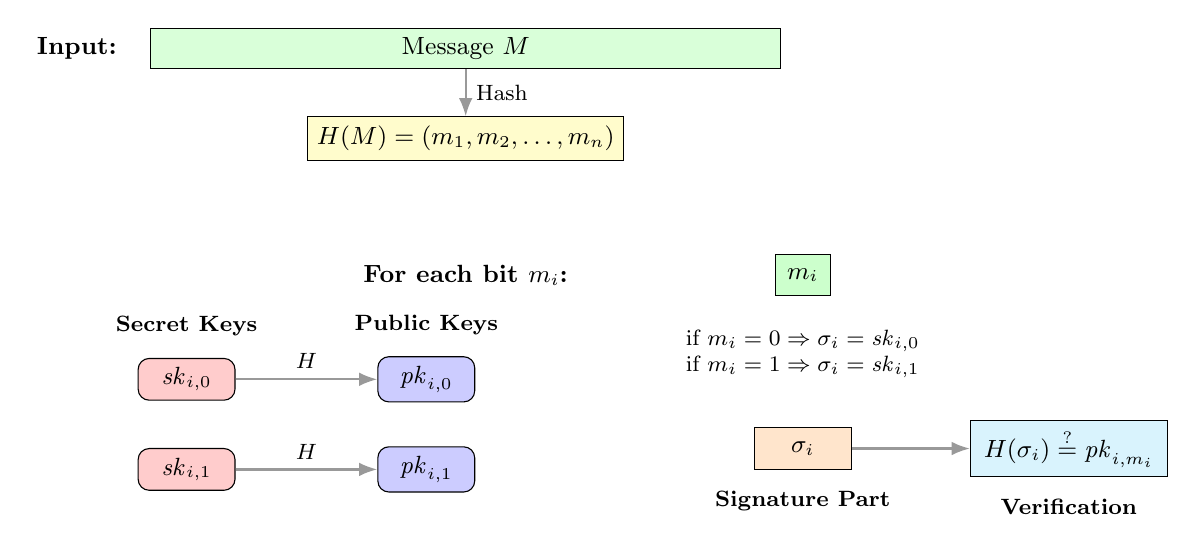
\begin{tikzpicture}[
    node distance=0.9cm and 1.8cm,
    secret/.style={rectangle, draw, rounded corners, fill=red!20, minimum height=1.5em, minimum width=3.5em, font=\small},
    public/.style={rectangle, draw, rounded corners, fill=blue!20, minimum height=1.5em, minimum width=3.5em, font=\small},
    msg/.style={rectangle, draw, fill=green!20, minimum height=1.5em, minimum width=2em, font=\small},
    sig/.style={rectangle, draw, fill=orange!20, minimum height=1.5em, minimum width=3.5em, font=\small},
    arrow/.style={-Latex, thick, draw=gray!80},
    label/.style={font=\footnotesize}
]

% --- Message ---
\node[rectangle, draw, fill=green!15, minimum width=8cm, minimum height=1.2em, font=\small] (msgbox) {Message $M$};
\node[left=0.3cm of msgbox, font=\small\bfseries] {Input:};

% --- Hash ---
\node[rectangle, draw, fill=yellow!20, below=0.6cm of msgbox, minimum width=3cm, font=\small] (hashM) {$H(M) = (m_1, m_2, \ldots, m_n)$};
\draw[arrow] (msgbox) -- (hashM) node[midway, right, font=\footnotesize] {Hash};

% --- Bit i key pairs ---
\node[below=1.2cm of hashM, font=\small\bfseries] (bitlabel) {For each bit $m_i$:};

% Secret keys
\node[secret, below left=0.8cm and 1.5cm of bitlabel] (sk0) {$\mathit{sk}_{i,0}$};
\node[secret, below=0.6cm of sk0] (sk1) {$\mathit{sk}_{i,1}$};
\node[above=0.15cm of sk0, font=\footnotesize\bfseries] {Secret Keys};

% Public keys
\node[public, right=1.8cm of sk0] (pk0) {$\mathit{pk}_{i,0}$};
\node[public, right=1.8cm of sk1] (pk1) {$\mathit{pk}_{i,1}$};
\node[above=0.15cm of pk0, font=\footnotesize\bfseries] {Public Keys};

% Hash arrows
\draw[arrow] (sk0) -- (pk0) node[midway, above, font=\footnotesize] {$H$};
\draw[arrow] (sk1) -- (pk1) node[midway, above, font=\footnotesize] {$H$};

% --- Signing ---
\node[msg, right=2.5cm of bitlabel] (mi) {$m_i$};
\node[below=0.3cm of mi, font=\footnotesize, text width=3cm, align=center] (rule) {if $m_i=0 \Rightarrow \sigma_i = \mathit{sk}_{i,0}$\\if $m_i=1 \Rightarrow \sigma_i = \mathit{sk}_{i,1}$};

% --- Signature output ---
\node[sig, below=0.5cm of rule] (sigout) {$\sigma_i$};
\node[below=0.15cm of sigout, font=\footnotesize\bfseries] {Signature Part};

% --- Verification ---
\node[rectangle, draw, fill=cyan!15, right=1.5cm of sigout, minimum width=2.5cm, minimum height=1.8em, font=\small] (verify) {$H(\sigma_i) \stackrel{?}{=} \mathit{pk}_{i,m_i}$};
\node[below=0.15cm of verify, font=\footnotesize\bfseries] {Verification};

\draw[arrow] (sigout) -- (verify);

\end{tikzpicture}
\caption{Lamport signature scheme for bit position $i$. The message $M$ is first hashed to obtain the bit string $(m_1, \ldots, m_n)$. For each bit $m_i$, the signer selects the corresponding secret key $\mathit{sk}_{i,m_i}$ as the signature component $\sigma_i$. The verifier checks that $H(\sigma_i)$ equals the public key $\mathit{pk}_{i,m_i}$.}
\label{fig:lamport}
\end{figure}
The Lamport signature scheme \cite{lamport1979constructing} is the first known hash-based signature algorithm. This scheme generates signatures that can only be used once, hence requiring a different key pair for each message. The steps of the scheme are as follows:

\begin{subsubsection}{Lamport Key Generation}
    Let us assume that a 256-bit message will be signed. In the Lamport algorithm, each bit of the signature requires 2 keys, resulting in a total of 512 public and private keys. The private keys are generated randomly and grouped as follows:

    \[
    \text{sk}_0 = \text{sk}_{10}, \text{sk}_{20}, \ldots, \text{sk}_{2560}
    \]
    \[
    \text{sk}_1 = \text{sk}_{11}, \text{sk}_{21}, \ldots, \text{sk}_{2561}
    \]
    
    The public keys are obtained by applying a hash function to each private key:
    
    \[
    \text{pk}_0 = H(\text{sk}_{10}), H(\text{sk}_{20}), \ldots, H(\text{sk}_{2560})
    \]
    \[
    \text{pk}_1 = H(\text{sk}_{11}), H(\text{sk}_{21}), \ldots, H(\text{sk}_{2561}) \]
    
\end{subsubsection}

\begin{subsubsection}{Lamport Signature}

    Each bit of the message is examined. If the bit is 0, the corresponding part of the signature is taken from the \(\text{sk}_0\) group; if the bit is 1, it is taken from the \(\text{sk}_1\) group.

    For example, suppose the first three bits of our message are "001". Then, the first three parts of the signature would be:

    \[
    \text{sk}_{10} \| \text{sk}_{20} \| \text{sk}_{31}
    \]
    
\end{subsubsection}

\begin{subsubsection}{Signature Verification}

    The verifier examines each bit of the message one by one. If the bit value is 0, the hash of the corresponding part of the signature is computed and compared with the corresponding part of \(\text{pk}_0\). If the bit is 1, it is compared with the corresponding part of \(\text{pk}_1\).

    This process is repeated for all bits. If all comparisons are equal, then the signature is successfully verified.
    
\end{subsubsection}
    
\end{subsection}

\begin{subsection}{WOTS and WOTS+}

    The WOTS (Winternitz One-Time Signature) algorithm \cite{buchmann2013security}, like the Lamport signature algorithm, is a one-time signature scheme. While in the Lamport algorithm each bit of the message is signed individually, in the WOTS scheme the message is divided into chunks of \( w \) bits, and each chunk is signed instead of individual bits. 

    As a result, the number of signature components is reduced from $n$ (one per bit) to $\ell_1 = \lceil n / \log_2 w \rceil$, where $n$ is the message length in bits. However, a \( w \)-bit message chunk can take \( 2^w \) different values, and na\"ively one would need a separate private key for each possible value.

    This key-explosion problem is resolved using iterated hash chains: instead of storing $2^w$ distinct keys per chunk, a single secret key is hashed up to $w-1$ times, so that the $i$-th value in the chain corresponds to the chunk value $i$. Note that the security of WOTS requires an additional checksum to prevent an adversary from advancing hash chains; the checksum mechanism is described in Section~\ref{sec:Checksum}.

    \begin{subsubsection}{WOTS Key generation}

        Let us assume that the message is divided into \( N \) parts, each consisting of \( l \) bits. In this case, \( N \) secret keys \( \text{sk}_0, \text{sk}_1, \ldots, \text{sk}_N \) are randomly generated. The \( 2^l \) possible values that each part can take are obtained by applying a hash function repeatedly to the randomly generated keys.

        \begin{figure}[ht]
            \centering
            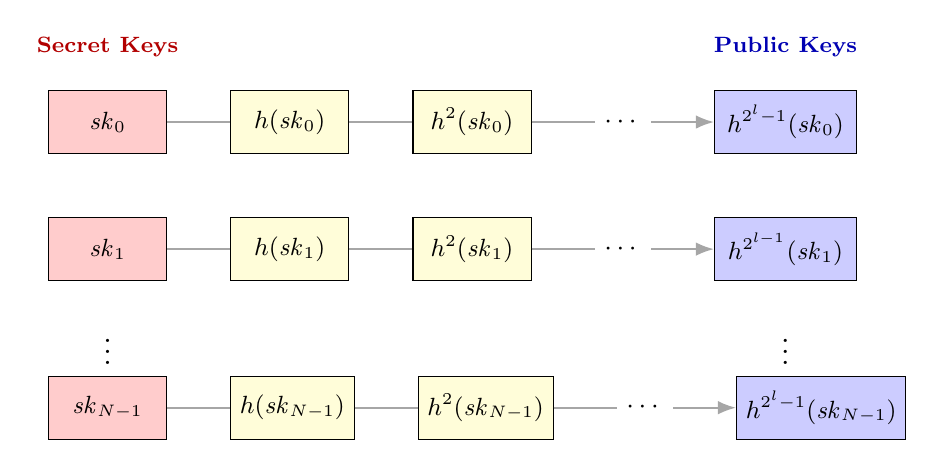
\begin{tikzpicture}[
        node distance=0.8cm and 0.8cm,
        sk/.style={draw, fill=red!20, minimum width=1.5cm, minimum height=0.8cm, align=center, font=\small},
        mid/.style={draw, fill=yellow!15, minimum width=1.5cm, minimum height=0.8cm, align=center, font=\small},
        pk/.style={draw, fill=blue!20, minimum width=1.8cm, minimum height=0.8cm, align=center, font=\small},
        arr/.style={-{Latex}, thick, gray!70}
      ]

      % Row 0
      \node[sk] (sk0) {$\mathit{sk}_0$};
      \node[mid,right=of sk0] (hsk0) {$h(\mathit{sk}_0)$};
      \node[mid,right=of hsk0] (h2sk0) {$h^2(\mathit{sk}_0)$};
      \node[right=of h2sk0] (dots0) {$\cdots$};
      \node[pk,right=of dots0] (h2i1sk0) {$h^{2^l-1}(\mathit{sk}_0)$};
      \draw[arr] (sk0)--(hsk0)--(h2sk0)--(dots0)--(h2i1sk0);

      % Row 1
      \node[sk,below=of sk0] (sk1) {$\mathit{sk}_1$};
      \node[mid,right=of sk1] (hsk1) {$h(\mathit{sk}_1)$};
      \node[mid,right=of hsk1] (h2sk1) {$h^2(\mathit{sk}_1)$};
      \node[right=of h2sk1] (dots1) {$\cdots$};
      \node[pk,right=of dots1] (h2i1sk1) {$h^{2^{l-1}}(\mathit{sk}_1)$};
      \draw[arr] (sk1)--(hsk1)--(h2sk1)--(dots1)--(h2i1sk1);

      % Vertical dots
      \node[below=0.4cm of sk1, font=\large] {$\vdots$};
      \node[below=0.4cm of h2i1sk1, font=\large] {$\vdots$};

      % Row N-1
      \node[sk,below=1.2cm of sk1] (skN) {$\mathit{sk}_{N-1}$};
      \node[mid,right=of skN] (hskN) {$h(\mathit{sk}_{N-1})$};
      \node[mid,right=of hskN] (h2skN) {$h^2(\mathit{sk}_{N-1})$};
      \node[right=of h2skN] (dotsN) {$\cdots$};
      \node[pk,right=of dotsN] (h2i1skN) {$h^{2^l-1}(\mathit{sk}_{N-1})$};
      \draw[arr] (skN)--(hskN)--(h2skN)--(dotsN)--(h2i1skN);

      % Column labels
      \node[above=0.3cm of sk0, font=\footnotesize\bfseries, red!70!black] {Secret Keys};
      \node[above=0.3cm of h2i1sk0, font=\footnotesize\bfseries, blue!70!black] {Public Keys};

        \end{tikzpicture}
            \caption{WOTS key generation. Each secret key $\mathit{sk}_i$ (red) is iteratively hashed to produce intermediate chain values (yellow) and the final public key component $h^{2^l-1}(\mathit{sk}_i)$ (blue).}
            \label{fig:WOTS}
        \end{figure}

        In Figure \ref{fig:WOTS}, the secret keys are shown. The public key is obtained by applying the hash function \( 2^l \) times to each secret key (i.e., the \( 2^l \)-th hash). 

        For example, if the value of the first message chunk is 0, then \(\text{sk}_0\) is used in the signature. If the value is \( 2^l - 1 \), then the signature value is \( h^{2^l - 1}(\text{sk}_0) \).

        
    \end{subsubsection}

    \begin{subsubsection}{WOTS Signature}

        For each part of the message, the appropriate number of hash iterations is applied to the corresponding secret key. These hashed values are concatenated to form the complete signature.

        For example, suppose the first three chunks of the message are:
        
        \[
        001 \| 010 \| 111
        \]
        
        Then the first three parts of the signature would be:
        
        \[
        h(\text{sk}_0) \| h^2(\text{sk}_1) \| h^7(\text{sk}_2)
        \]
                
    \end{subsubsection}

    \begin{subsubsection}{WOTS+ Signature Verification}

        The verifier examines each message part individually. By checking the numerical value of each chunk, the verifier determines how many hash iterations are needed to reach the public key. It then hashes the corresponding part of the signature that many times. The result is compared with the known public key. If all values match, the signature is considered valid.
        
    \end{subsubsection}

    \begin{subsubsection}{WOTS+ \cite{cryptoeprint:2017/965}}

        WOTS+ is an improved variant of WOTS that introduces a randomized \emph{chaining function}. The chaining function $c_k$ defines a single step in the hash chain and is given by:
        \[
        c_k(x, r) = H\bigl(x \oplus r_k\bigr)
        \]
        where $H$ is the underlying hash function, $x$ is the current chain value, and $r_k$ is a pseudorandom bitmask derived from the public seed and the address structure for step $k$. The full chain of length $s$ starting from value $x_0$ is computed as:
        \[
        c^s(x_0) = c_s\bigl(c_{s-1}\bigl(\cdots c_1(x_0, r_1)\cdots, r_{s-1}\bigr), r_s\bigr)
        \]
        This randomized masking serves two critical purposes: (1)~it provides \emph{domain separation}, ensuring that each hash evaluation within the scheme operates on a distinct, position-dependent input even when the underlying data coincides, and (2)~it mitigates \emph{multi-target attacks} by preventing an adversary from amortizing preimage searches across multiple hash chain positions.
        
    \end{subsubsection}
    
    
\end{subsection}


\begin{subsection}{Merkle Trees and Multi-Signatures}

Lamport and WOTS schemes are one-time signature algorithms, meaning they allow signing only a single message with generated keys. However, in practical scenarios, signature algorithms are expected to support multiple signatures. To convert one-time signature schemes into algorithms that can sign multiple messages, \textbf{Merkle trees} are used.

As an example, the WOTS+ scheme can be used together with a Merkle tree. Figure \ref{fig:Merkle} shows the sketch of a Merkle tree used with WOTS+. The bottom leaves of the Merkle tree are the hash values of the WOTS+ public keys. Using a Merkle tree of height \( h \), a signature scheme capable of signing \( 2^h \) messages can be constructed.

In addition to increasing signature capacity, Merkle trees also have the advantage of \textbf{reducing public key size}. Normally, a WOTS+ public key consists of multiple components—one for each message chunk—but when used with a Merkle tree, only \textbf{one public key} is required: the root of the Merkle tree. To verify a signature, the verifier must access certain intermediate nodes of the Merkle tree in order to compute the root. These intermediate values can be included as part of the signature, thus enabling successful verification.

\begin{figure}[h]
    \centering
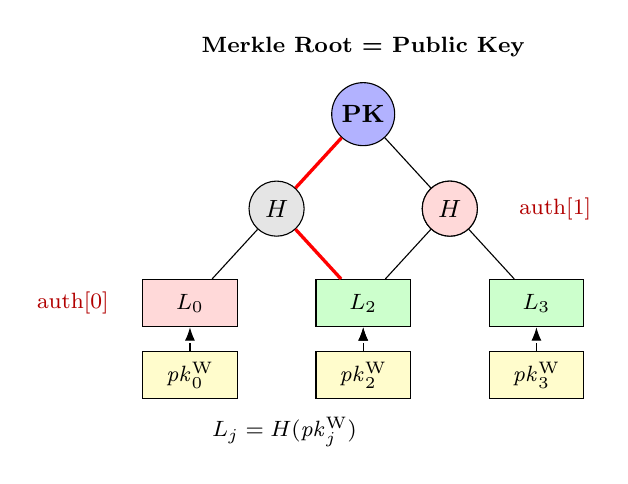
\begin{tikzpicture}[
    level distance=1.2cm,
    sibling distance=2.2cm,
    every node/.style={font=\small},
    hash_node/.style={circle, draw, fill=gray!20, minimum size=0.7cm, inner sep=1pt},
    root_node/.style={circle, draw, fill=blue!30, minimum size=0.8cm, inner sep=1pt, font=\small\bfseries},
    leaf_node/.style={rectangle, draw, fill=green!20, minimum width=1.2cm, minimum height=0.6cm, font=\footnotesize},
    wots_node/.style={rectangle, draw, fill=yellow!20, minimum width=1.2cm, minimum height=0.6cm, font=\footnotesize},
    edge from parent/.style={draw, -},
    auth/.style={draw, red, very thick}
]

% Root
\node[root_node] (root) {PK}
    child {
        node[hash_node] (h01) {$H$}
        child {
            node[leaf_node] (l0) {$L_0$}
        }
        child {
            node[leaf_node] (l1) {$L_1$}
        }
    }
    child {
        node[hash_node] (h23) {$H$}
        child {
            node[leaf_node] (l2) {$L_2$}
        }
        child {
            node[leaf_node] (l3) {$L_3$}
        }
    };

% WOTS+ public keys below leaves
\node[wots_node, below=0.3cm of l0] (w0) {$\mathit{pk}^{\text{W}}_0$};
\node[wots_node, below=0.3cm of l1] (w1) {$\mathit{pk}^{\text{W}}_1$};
\node[wots_node, below=0.3cm of l2] (w2) {$\mathit{pk}^{\text{W}}_2$};
\node[wots_node, below=0.3cm of l3] (w3) {$\mathit{pk}^{\text{W}}_3$};

\draw[-Latex, dashed] (w0) -- (l0);
\draw[-Latex, dashed] (w1) -- (l1);
\draw[-Latex, dashed] (w2) -- (l2);
\draw[-Latex, dashed] (w3) -- (l3);

% Labels
\node[above=0.2cm of root, font=\footnotesize\bfseries] {Merkle Root = Public Key};
\node[below=0.1cm of w1, font=\footnotesize, xshift=-1cm] {$L_j = H(\mathit{pk}^{\text{W}}_j)$};

% Authentication path highlight (for signing leaf 1)
\draw[auth] (l1) -- (h01);
\draw[auth] (h01) -- (root);
\node[leaf_node, fill=red!15, minimum width=1.2cm] at (l0) {$L_0$};
\node[hash_node, fill=red!15] at (h23) {$H$};
\node[left=0.3cm of l0, font=\footnotesize, text=red!70!black] {auth[0]};
\node[right=0.4cm of h23, font=\footnotesize, text=red!70!black] {auth[1]};

\end{tikzpicture}
    \caption{Merkle tree of height $h=2$ used with WOTS+. Each leaf $L_j$ is the hash of the corresponding WOTS+ public key $\mathit{pk}^{\text{W}}_j$. The root serves as the overall public key. When signing with leaf~1, the authentication path (highlighted in red) consists of sibling nodes $L_0$ and $H(L_2 \| L_3)$, which the verifier uses to reconstruct the root.}
    \label{fig:Merkle}
\end{figure}

\end{subsection}

\begin{subsection}{L-tree and Hashing public key}{\label{sec:L-tree}}

    When combining one-time signature schemes with a Merkle tree, the public key of the one-time signature scheme is selected as the bottom leaf of the Merkle tree. However, in the WOTS algorithm, a single signature includes not one but multiple public key components—one for each message part.
    
    To resolve this issue, two different approaches are employed:
    
    \begin{enumerate}
        \item \textbf{L-tree (used in XMSS):} The L-tree is a specialized Merkle tree used to compress multiple public key components into a single public key. It repeatedly hashes pairs of public key elements until only one remains.
    
        \item \textbf{Hashing (used in SPHINCS+):} In this method, all public key components are concatenated, and a single hash value is computed over the entire concatenation. This resulting hash serves as the single public key for Merkle tree integration.
    \end{enumerate}

    
\end{subsection}

\begin{subsection}{Base-\texorpdfstring{$w$}{w} Representation }

In hash-based signature schemes such as WOTS and XMSS, the message digest is first transformed into a base-$w$ representation before signing. This \textbf{base-$w$ representation} is a critical component of the signing process and directly influences the structure and security of the signature.

The main purposes of using base-$w$ representation are to:

\begin{itemize}
    \item reduce the size of the signature compared to bit-wise representations (as in the Lamport scheme),
    \item represent the message digest in a form suitable for the Winternitz one-time signature construction,
    \item control the number of hash iterations per key chain in WOTS+,
    \item and balance the trade-off between performance (speed) and signature length through the choice of $w$.
\end{itemize}

Let the hash function produce an output of $n$ \emph{bytes} (i.e., $8n$ bits).\footnote{In the XMSS and SPHINCS+ specifications, $n$ denotes the security parameter in \emph{bytes}, not bits. Hence the factor of~8 in the numerator converts bytes to bits.} The number of base-$w$ digits required to represent this $8n$-bit message digest is:
\[
\ell_1 = \left\lceil \frac{8n}{\log_2 w} \right\rceil
\]
Each digit in this representation is an integer in the range $[0, w-1]$, and indicates how many times the corresponding chain of the private key should be hashed to produce the signature component.

\textbf{Example:}  
Suppose $n = 256$ and $w = 16$. Then:
\[
\ell_1 = \left\lceil \frac{8 \cdot 256}{\log_2 16} \right\rceil = \left\lceil \frac{2048}{4} \right\rceil = 512
\]
So, the hash output will be split into 512 base-$16$ digits.

After computing the base-$w$ representation of the message digest, a checksum is computed and appended (as described in the section \ref{sec:Checksum}), forming the complete message input for WOTS+.

The choice of $w$ is significant: 
\begin{itemize}
    \item A smaller $w$ increases the number of digits $\ell_1$ (and thus the signature size) but reduces the number of hash computations.
    \item A larger $w$ reduces the signature size but requires more hash computations per signature, increasing signing and verification time.
\end{itemize}

In summary, the base-$w$ representation enables the WOTS+ signature scheme to efficiently encode the message digest while maintaining flexibility across a range of parameter choices.

\end{subsection}


\begin{subsection}{Checksum}{\label{sec:Checksum}}

In hash-based signature algorithms such as WOTS and XMSS, the message to be signed is first encoded into a base-$w$ representation. However, this encoding alone is not sufficient to ensure existential unforgeability (EUF-CMA security, see Section~2.2). Specifically, without additional protection, an adversary who observes a valid signature $\sigma$ for message $M$ could construct a valid signature for a \emph{different} message $M'$ by simply advancing the hash chains: if a base-$w$ digit $m_i$ is replaced by $m'_i > m_i$, the adversary can compute $h^{m'_i - m_i}(\sigma_i)$ to obtain the corresponding signature component. To prevent this \textbf{hash chain advancement attack}, a \textbf{checksum} value is appended to the base-$w$ representation of the message. This checksum serves to:

\begin{itemize}
    \item prevent attacks that attempt to alter message chunks by increasing or decreasing hash iterations,
    \item protect against fault injection attacks that aim to exploit the absence or corruption of the checksum,
    \item and detect message modifications or signature reuse.
\end{itemize}

The checksum is calculated by summing the differences between the maximum possible chunk value $(w-1)$ and each base-$w$ digit of the message. If the message is represented by $m_0, m_1, \ldots, m_{\ell_1-1}$ in base-$w$, the checksum $c$ is given by:
\[
c = \sum_{i=0}^{\ell_1-1} (w - 1 - m_i)
\]
This value is then encoded into base-$w$ as an additional sequence of digits, forming the checksum part of the message. The total number of checksum digits required is $\ell_2$, calculated as:
\[
\ell_2 = \left\lfloor \frac{\log_2(\ell_1(w-1))}{\log_2 w} \right\rfloor + 1
\]

As a result, the full message to be signed by WOTS+ consists of $\ell = \ell_1 + \ell_2$ base-$w$ digits. Each digit corresponds to the number of hash function applications to be performed on a particular chain of the private key.

\textbf{The checksum} plays a crucial role in maintaining the integrity and one-time nature of the WOTS+ signature. Without it, an attacker could transform a valid signature for one message into a valid signature for another message by manipulating the hash chains, which would compromise the existential unforgeability of the scheme.

\end{subsection}


\begin{subsection}{FORS}

    The \textbf{FORS algorithm} (Forest of Random Subsets) \cite{bernstein2019sphincs+} is a \textit{few-time signature scheme} that serves as a critical building block in SPHINCS+ (SLH-DSA). It is used specifically at the \emph{bottom layer} of the SPHINCS+ hypertree, where the signed data is a message digest rather than the root of another tree.

    \subsubsection{Why FORS Instead of WOTS+ at the Bottom Layer}

    In SPHINCS+, all layers above the bottom use WOTS+ instances to sign the roots of the subtrees below them. However, at the bottom layer, the scheme must sign a \emph{message digest}. WOTS+ is a strict one-time signature: reusing a WOTS+ key pair to sign two different messages immediately leaks information that can be exploited to forge signatures. Since SPHINCS+ is stateless, it selects the signing leaf index pseudorandomly (based on a hash of the message), and there is a non-zero probability that the same leaf is selected more than once across different signing operations. FORS tolerates this because it is a \emph{few-time} signature scheme: even if the same FORS instance signs a small number of different messages, the security degradation remains bounded and acceptable for the overall scheme's security proof.

    \subsubsection{FORS Construction}

    FORS is parameterized by two values: the number of trees $k$ and the height $a$ of each tree (so each tree has $2^a$ leaves). The message digest to be signed is split into $k$ chunks, each of $a$ bits, yielding $k$ integer indices $i_0, i_1, \ldots, i_{k-1}$, where each $i_j \in \{0, 1, \ldots, 2^a - 1\}$.

    \textbf{Key Generation.}  
    For each of the $k$ trees, $2^a$ secret key values are generated (derived deterministically from a seed and an address structure). The leaves of each tree are computed by hashing the corresponding secret keys. A binary Merkle tree is then built over these $2^a$ leaves, yielding a root for each tree. The $k$ tree roots are combined (e.g., by hashing their concatenation) to produce the overall FORS public key.

    \textbf{Signing.}  
    Given the $k$ indices $(i_0, \ldots, i_{k-1})$ derived from the message digest, the FORS signature consists of, for each tree $j$:
    \begin{itemize}
        \item the secret key value $\mathit{sk}_{j, i_j}$ at position $i_j$ in tree $j$, and
        \item the authentication path (the $a$ sibling nodes along the path from leaf $i_j$ to the root of tree $j$).
    \end{itemize}

    \textbf{Verification.}  
    For each tree $j$, the verifier hashes the provided secret key to obtain the leaf, then uses the authentication path to reconstruct the tree root. All $k$ reconstructed roots are combined and compared against the known FORS public key.

    \subsubsection{Example}

    Consider FORS with $k = 4$ trees of height $a = 3$ (so each tree has $2^3 = 8$ leaves). Suppose the message digest yields the following four 3-bit chunks:
    
    \[100 \quad 011 \quad 101 \quad 000\]

    This means: in tree~0, select leaf~4 ($100_2$); in tree~1, select leaf~3 ($011_2$); in tree~2, select leaf~5 ($101_2$); in tree~3, select leaf~0 ($000_2$). Figure~\ref{fig:FORS} illustrates the resulting signature structure.
    
    \begin{figure}[ht]
    \centering
    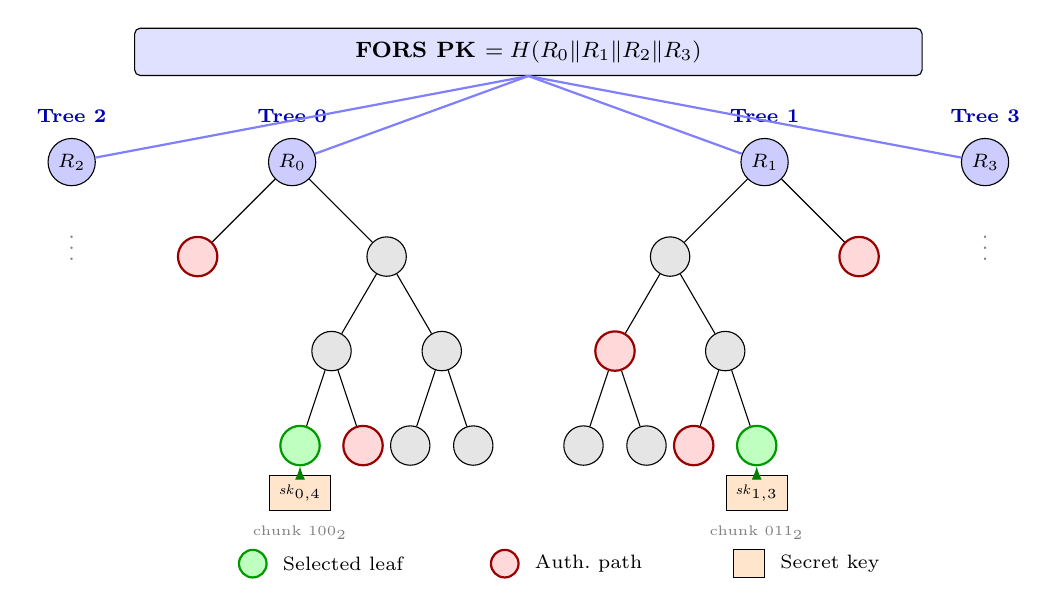
\begin{tikzpicture}[
        hn/.style={circle, draw, fill=gray!20, minimum size=5mm, inner sep=0pt, font=\scriptsize},
        sel/.style={circle, draw=green!60!black, fill=green!25, minimum size=5mm, inner sep=0pt, font=\scriptsize, thick},
        auth/.style={circle, draw=red!60!black, fill=red!15, minimum size=5mm, inner sep=0pt, font=\scriptsize, thick},
        rn/.style={circle, draw, fill=blue!20, minimum size=6mm, inner sep=0pt, font=\scriptsize\bfseries},
        skn/.style={rectangle, draw, fill=orange!20, minimum width=6mm, minimum height=4mm, font=\tiny}
    ]

    %% ---- FORS PK box ----
    \node[rectangle, draw, fill=blue!12, minimum width=10cm, minimum height=6mm,
          font=\footnotesize\bfseries, rounded corners=2pt] (fpk) at (0,0)
          {FORS PK $= H(R_0 \| R_1 \| R_2 \| R_3)$};

    %% ======== Tree 0  (idx=4, chunk 100) ========
    \node[rn] (r0) at (-3,-1.4) {$R_0$};
    \draw[thick, blue!50] (r0) -- (fpk.south);
    \node[above=2pt of r0, font=\scriptsize\bfseries, blue!70!black] {Tree 0};
    % level 1
    \node[auth] (a0) at (-4.2,-2.6) {};
    \node[hn]   (b0) at (-1.8,-2.6) {};
    \draw (r0)--(a0) (r0)--(b0);
    % level 2
    \node[hn]   (c0) at (-2.5,-3.8) {};
    \node[hn]   (d0) at (-1.1,-3.8) {};
    \draw (b0)--(c0) (b0)--(d0);
    % level 3 (leaves)
    \node[sel] (e0) at (-2.9,-5.0) {};
    \node[auth](f0) at (-2.1,-5.0) {};
    \node[hn]  (g0) at (-1.5,-5.0) {};
    \node[hn]  (h0) at (-0.7,-5.0) {};
    \draw (c0)--(e0) (c0)--(f0) (d0)--(g0) (d0)--(h0);
    % sk
    \node[skn, below=3pt of e0] (sk0) {$\mathit{sk}_{0,4}$};
    \draw[-Latex, green!50!black] (sk0)--(e0);
    \node[below=2pt of sk0, font=\tiny, gray] {chunk $100_2$};

    %% ======== Tree 1  (idx=3, chunk 011) ========
    \node[rn] (r1) at (3,-1.4) {$R_1$};
    \draw[thick, blue!50] (r1) -- (fpk.south);
    \node[above=2pt of r1, font=\scriptsize\bfseries, blue!70!black] {Tree 1};
    % level 1
    \node[hn]   (a1) at (1.8,-2.6) {};
    \node[auth] (b1) at (4.2,-2.6) {};
    \draw (r1)--(a1) (r1)--(b1);
    % level 2
    \node[auth] (c1) at (1.1,-3.8) {};
    \node[hn]   (d1) at (2.5,-3.8) {};
    \draw (a1)--(c1) (a1)--(d1);
    % level 3 (leaves)
    \node[hn]  (e1) at (0.7,-5.0) {};
    \node[hn]  (f1) at (1.5,-5.0) {};
    \node[auth](g1) at (2.1,-5.0) {};
    \node[sel] (h1) at (2.9,-5.0) {};
    \draw (c1)--(e1) (c1)--(f1) (d1)--(g1) (d1)--(h1);
    % sk
    \node[skn, below=3pt of h1] (sk1) {$\mathit{sk}_{1,3}$};
    \draw[-Latex, green!50!black] (sk1)--(h1);
    \node[below=2pt of sk1, font=\tiny, gray] {chunk $011_2$};

    %% ======== Tree 2 and Tree 3 (root-only) ========
    \node[rn] (r2) at (-5.8,-1.4) {$R_2$};
    \node[rn] (r3) at (5.8,-1.4) {$R_3$};
    \draw[thick, blue!50] (r2)--(fpk.south) (r3)--(fpk.south);
    \node[below=3mm of r2, font=\footnotesize, gray] {$\vdots$};
    \node[below=3mm of r3, font=\footnotesize, gray] {$\vdots$};
    \node[above=2pt of r2, font=\scriptsize\bfseries, blue!70!black] {Tree 2};
    \node[above=2pt of r3, font=\scriptsize\bfseries, blue!70!black] {Tree 3};

    %% ---- Legend ----
    \node[sel, minimum size=3.5mm] (lg1) at (-3.5,-6.5) {};
    \node[right=2pt of lg1, font=\scriptsize] {Selected leaf};
    \node[auth, minimum size=3.5mm] (lg2) at (-0.3,-6.5) {};
    \node[right=2pt of lg2, font=\scriptsize] {Auth.\ path};
    \node[skn, minimum width=4mm, minimum height=3.5mm] (lg3) at (2.8,-6.5) {};
    \node[right=2pt of lg3, font=\scriptsize] {Secret key};

    \end{tikzpicture}
    \caption{FORS signature example with $k = 4$ trees, each of height $a = 3$. Trees~0 and~1 are shown in detail: the message digest chunk selects a leaf index (green), and the authentication path siblings (red) are included in the signature along with the secret key $\mathit{sk}_{i,\mathit{idx}}$. All four tree roots $R_0, \ldots, R_3$ are hashed together to form the FORS public key.}
    \label{fig:FORS}
    \end{figure}

\end{subsection}

\begin{subsection}{Comparison of OTS and FTS Building Blocks}

Table~\ref{tab:ots_comparison} compares the one-time and few-time signature schemes discussed above. Understanding the trade-offs between these building blocks explains why specific components are chosen for different standardized schemes: WOTS+ is used in XMSS, LMS, and the upper layers of SPHINCS+ due to its compact signatures, while FORS is used at the bottom layer of SPHINCS+ because it tolerates limited key reuse.

\begin{table}[ht]
\centering
\renewcommand{\arraystretch}{1.3}
\caption{Comparison of one-time and few-time signature building blocks}
\label{tab:ots_comparison}
\begin{tabular}{|l|c|c|c|c|}
\hline
\textbf{Property} & \textbf{Lamport} & \textbf{WOTS} & \textbf{WOTS+} & \textbf{FORS} \\
\hline
\textbf{Type} & OTS & OTS & OTS & FTS \\
\hline
\textbf{Sig.\ components} & $2n$ & $\ell$ & $\ell$ & $k(a+1)$ \\
\hline
\textbf{Sig.\ size} & $2n \cdot n$ & $\ell \cdot n$ & $\ell \cdot n$ & $k(a+1) \cdot n$ \\
\hline
\textbf{Hash calls (sign)} & $0$ & $\sum m_i$ & $\sum m_i$ & $k$ (+ auth) \\
\hline
\textbf{Checksum} & No & Yes & Yes & No \\
\hline
\textbf{Randomization} & None & None & XOR bitmask & Tweakable \\
\hline
\textbf{Multi-target} & Vulnerable & Vulnerable & Resistant & Resistant \\
\hline
\textbf{Key reuse} & Insecure & Insecure & Insecure & Bounded \\
\hline
\textbf{Used in} & (Historical) & -- & XMSS, LMS, SPHINCS+ & SPHINCS+ \\
\hline
\end{tabular}
\end{table}

Here, $n$ is the security parameter (hash output length), $\ell = \ell_1 + \ell_2$ is the total number of WOTS/WOTS+ chains, $k$ is the number of FORS trees, and $a$ is the height of each FORS tree.

\end{subsection}

\begin{subsection}{Address Structures in Hash-Based Signature Schemes}
    Hash-based signature schemes consist of either very large Merkle trees or multi-layered Merkle trees in order to increase their signature capacity. Since the same hash function is repeatedly used within the tree and similar operations are performed, \textbf{address structures} are used in hash-based signature schemes to:
\begin{itemize}
    \item distinguish each operation,
    \item determine the position within the tree,
    \item track how many hash operations have been applied,
    \item and provide input differentiation for the hash functions.
\end{itemize}

\textbf{Table} \ref{tab: Adress} shows the \textbf{OTS address structure} used in the XMSS algorithm \cite{huelsing2018rfc}. In the example structure, the following fields appear in order from top to bottom:
\begin{itemize}
    \item the layer in the multi-tree,
    \item the specific tree identifier,
    \item address type (e.g., OTS),
    \item index of the L-tree–WOTS pair,
    \item WOTS chain identifier,
    \item index of the hash operation within the chain,
    \item a flag indicating whether the hash value is used for encryption or masking.
\end{itemize}

Depending on the algorithm and its internal structure, the format of the address field can vary.


\begin{table}[H]
\centering
\renewcommand{\arraystretch}{1.5}
\begin{tabular}{|c|c|}
\hline
\textbf{Field} & \textbf{Size} \\
\hline
layer address     & 32 bits \\
\hline
tree address      & 64 bits \\
\hline
type = 0          & 32 bits \\
\hline
OTS address       & 32 bits \\
\hline
chain address     & 32 bits \\
\hline
hash address      & 32 bits \\
\hline
keyAndMask        & 32 bits \\
\hline
\end{tabular}
\caption{XMSS OTS Address Format}
\label{tab: Adress}
\end{table}

\end{subsection}

\begin{subsection}{Stateful and Stateless Hash-Based Signature Schemes}

    Hash-based signature algorithms can be categorized into two types: \textbf{stateful} and \textbf{stateless}. The fundamental difference between these two categories lies in the management of state information during the signature generation and verification processes.

\textbf{Stateful hash-based signature algorithms} require the maintenance of state information while generating signatures. These algorithms rely on \textit{one-time keys} that can be used only once per signature operation. Reusing these keys leads to serious security vulnerabilities. A representative example of such an algorithm is XMSS \cite{huelsing2018rfc}.

\textbf{Stateless hash-based signature algorithms}, in contrast, do not require any state information to be stored during the signing process. A prominent example of a stateless algorithm is SPHINCS+ \cite{bernstein2019sphincs+}.
    
\end{subsection}

\end{section}

\begin{section}{XMSS and \texorpdfstring{$XMSS^{MT}$}{XMSS MT}}

    In this section, the XMSS/\texorpdfstring{$XMSS^{MT}$}{XMSS MT} algorithms, as defined in the documents \cite{cooper2020recommendation} \cite{huelsing2018rfc}, will be explained using the fundamental structures presented in Section \ref{sec1}. The architecture of XMSS is given in Figure \ref{fig:xmss}.

\begin{figure}[h]
\centering
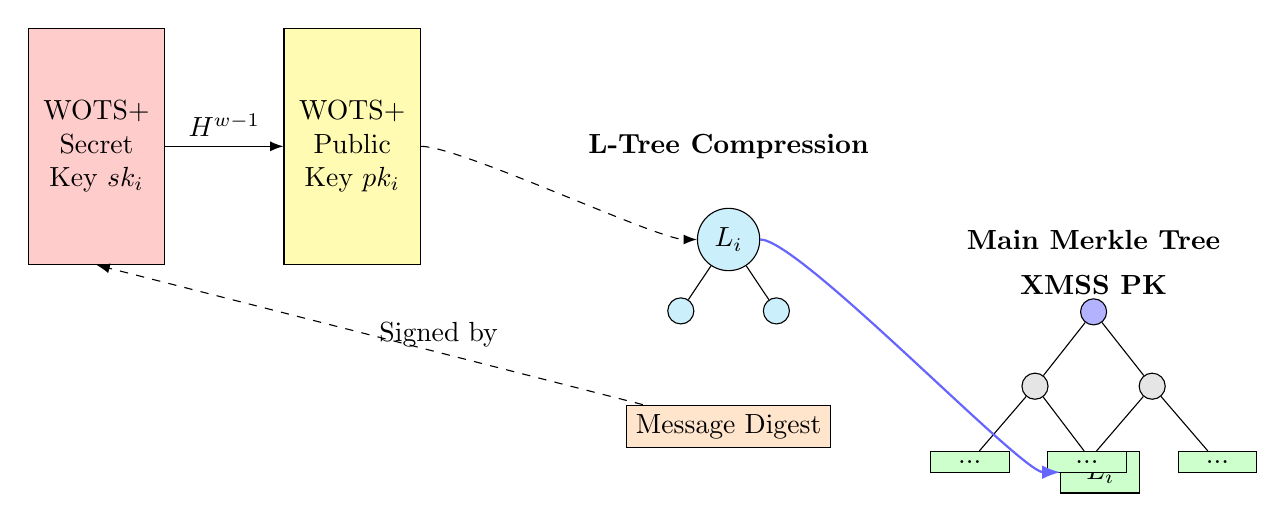
\begin{tikzpicture}[
    node distance=1.5cm,
    wots_pk/.style={rectangle, draw, fill=yellow!30, text width=1.5cm, align=center, minimum height=3cm},
    wots_sk/.style={rectangle, draw, fill=red!20, text width=1.5cm, align=center, minimum height=3cm},
    ltree_node/.style={circle, draw, fill=cyan!20},
    merkle_node/.style={circle, draw, fill=gray!20},
    leaf_node/.style={rectangle, draw, fill=green!20, minimum width=1cm},
    main_root/.style={merkle_node, fill=blue!30, label={[label distance=-2pt]90:\textbf{XMSS PK}}}
]

% WOTS+ Part
\node[wots_sk] (wots_sk) {WOTS+ Secret Key $sk_i$};
\node[wots_pk, right=of wots_sk] (wots_pk) {WOTS+ Public Key $pk_i$};
\draw[-Latex] (wots_sk) -- (wots_pk) node[midway, above] {$H^{w-1}$};

% L-Tree Part
\node[right=2cm of wots_pk] (ltree_label) {\textbf{L-Tree Compression}};
\node[ltree_node, below=0.5cm of ltree_label] (ltree_root) {$L_i$};
\node[ltree_node, below left=0.5cm and 0.2cm of ltree_root] (ltree1) {};
\node[ltree_node, below right=0.5cm and 0.2cm of ltree_root] (ltree2) {};
\draw (ltree1) -- (ltree_root) -- (ltree2);
\draw[-Latex, dashed] (wots_pk.east) .. controls +(0.5,0) and +(-0.5,0) .. (ltree_root.west);

% Merkle Tree Part
\node[right=2.5cm of ltree_root] (mt_label) {\textbf{Main Merkle Tree}};
\node[main_root, below=0.5cm of mt_label] (root) {};
\node[merkle_node, below left=0.7cm and 0.5cm of root] (n1) {};
\node[merkle_node, below right=0.7cm and 0.5cm of root] (n2) {};
\node[leaf_node, below left=0.7cm and 0.2cm of n1] (L0) {...};
\node[leaf_node, below right=0.7cm and 0.2cm of n1] (Li) {$L_i$};
\node[leaf_node, below left=0.7cm and 0.2cm of n2] (Lj) {...};
\node[leaf_node, below right=0.7cm and 0.2cm of n2] (LN) {...};
\draw (root) -- (n1) -- (L0);
\draw (n1) -- (Li);
\draw (root) -- (n2) -- (Lj);
\draw (n2) -- (LN);

% Connection from L-Tree to Merkle Tree
\draw[-Latex, thick, blue!60] (ltree_root.east) .. controls +(0.5,0) and +(-0.5,0) .. (Li.west);

% Signing part
\node[rectangle, draw, fill=orange!20, below=3cm of ltree_label] (msg) {Message Digest};
\draw[-Latex, dashed] (msg) -- (wots_sk.south) node[midway, right, text width=2cm] {Signed by};

\end{tikzpicture}
\caption{The architecture of XMSS. A WOTS+ secret key $\mathit{sk}_i$ (consisting of $\ell$ random $n$-byte strings) is used to sign a message digest. The corresponding WOTS+ public key $\mathit{pk}_i$ (obtained by hashing each chain $w{-}1$ times) is compressed via an L-Tree into a single leaf $L_i$. This leaf is placed in a Merkle tree of height $h$, whose root serves as the overall XMSS public key.}
\label{fig:xmss}
\end{figure}


    \begin{subsection}{XMSS Key Generation}

        In Algorithm \ref{alg:XMSS_keygen}, a pseudo-code representation of the key generation process of the \textbf{XMSS} algorithm is provided. First, the \textbf{WOTS+} private keys are generated. These keys can be created either completely at random or by passing a seed value through a key generation function. If all keys are generated randomly, they must be stored in memory for the signing process. However, since storing all the keys in memory is not realistic, this method is generally not used. Next, certain seed values are generated to be used throughout the algorithm, and the hash values of the WOTS+ private keys are taken to produce the WOTS+ public keys. In the pseudo-code, the value \texttt{idx} at the beginning of the \texttt{SK} section represents the state information (the index of the next unused OTS key pair).

        The key functions used in the algorithm are:
        \begin{itemize}
            \item \texttt{WOTS\_genSK()}: Generates a WOTS+ secret key, consisting of $\ell$ random $n$-byte strings (one per hash chain).
            \item \texttt{setSK\_PRF(SK, SK\_PRF)}: Stores the pseudorandom function key \texttt{SK\_PRF} (an $n$-byte string) into the private key structure. This key is used during signing to generate randomized message hashes.
            \item \texttt{setSEED(SK, SEED)}: Stores the public seed \texttt{SEED} (an $n$-byte string) in the key structure. The seed is used as a public parameter for all hash computations (bitmasks, address-based hashing).
            \item \texttt{treeHash(SK, s, t, ADRS)}: Computes the root of the Merkle subtree starting at leaf index $s$ with height $t$, using the WOTS+ public keys as leaves (after L-tree compression). The address structure \texttt{ADRS} tracks the position within the tree hierarchy.
            \item \texttt{toByte(x, y)}: Converts the integer $x$ into a $y$-byte string.
        \end{itemize}

        \begin{algorithm}
\caption{XMSS\_keyGen -- Generate an XMSS key pair}
\label{alg:XMSS_keygen}

\textbf{Input:} None \\
\textbf{Output:} XMSS private key \texttt{SK}, XMSS public key \texttt{PK}

\vspace{0.3cm}

\begin{tabular}{ll}
1: & \textit{// Example initialization for SK-specific contents} \\
2: & \texttt{idx} $\leftarrow 0$ \\
3: & \textbf{for} $i = 0$ \textbf{to} $2^h - 1$ \textbf{do} \\
4: & \quad \texttt{wots\_sk[i]} $\leftarrow$ \texttt{WOTS\_genSK()} \\
5: & \textbf{end for} \\
6: & Initialize \texttt{SK\_PRF} with a uniformly random $n$-byte string \\
7: & \texttt{setSK\_PRF(SK, SK\_PRF)} \\
8: & \textit{// Initialization for common contents} \\
9: & Initialize \texttt{SEED} with a uniformly random $n$-byte string \\
10: & \texttt{setSEED(SK, SEED)} \\
11: & \texttt{setWOTS\_SK(SK, wots\_sk)} \\
12: & \texttt{ADRS} $\leftarrow$ \texttt{toByte(0, 32)} \\
13: & \texttt{root} $\leftarrow$ \texttt{treeHash(SK, 0, h, ADRS)} \\
14: & \texttt{SK} $\leftarrow$ \texttt{idx $\parallel$ wots\_sk $\parallel$ SK\_PRF $\parallel$ root $\parallel$ SEED} \\
15: & \texttt{PK} $\leftarrow$ \texttt{OID $\parallel$ root $\parallel$ SEED} \\
16: & \textbf{return} \texttt{SK $\parallel$ PK}
\end{tabular}

\end{algorithm}

        
    \end{subsection}

    \begin{subsection}{XMSS Sign}

        In Algorithm \ref{alg:XMSS_sign}, the pseudo-code of the XMSS signing algorithm is presented. The \texttt{treeSig} function signs the message using WOTS and generates the authentication path required to reach the root of the tree. First, the state information is retrieved, then a random value is generated and concatenated with the message, after which a hash is computed from this combination. This hash value is then signed using the \texttt{treeSig} algorithm. The final signature consists of the concatenation of the state information, the random value, and the \texttt{treeSig} signature, respectively.


        \begin{algorithm}
\caption{XMSS\_sign – Generate an XMSS signature and update the XMSS private key}
\label{alg:XMSS_sign}

\textbf{Input:} Message $M$, XMSS private key $SK$ \\
\textbf{Output:} Updated $SK$, XMSS signature $Sig$

\vspace{0.3cm}

\begin{tabular}{ll}
1: & \texttt{idx\_sig} $\leftarrow$ \texttt{getIdx(SK)} \\
2: & \texttt{setIdx(SK, idx\_sig + 1)} \\
3: & \texttt{ADRS} $\leftarrow$ \texttt{toByte(0, 32)} \\
4: & \texttt{r} $\leftarrow$ \texttt{PRF(getSK\_PRF(SK), toByte(idx\_sig, 32))} \\
5: & \texttt{M'} $\leftarrow$ \texttt{H\_msg(r $\parallel$ getRoot(SK) $\parallel$ toByte(idx\_sig, n), M)} \\
6: & \texttt{Sig} $\leftarrow$ \texttt{idx\_sig $\parallel$ r $\parallel$ treeSig(M', SK, idx\_sig, ADRS)} \\
7: & \textbf{return} \texttt{SK $\parallel$ Sig}
\end{tabular}

\end{algorithm}

        
\end{subsection}

\begin{subsection}{XMSS Verify}

In Algorithm \ref{alg:xmss_rootfromSign} and \ref{alg:xmss_verify}, the pseudo-code of the XMSS signature verification is presented. First, the WOTS public key is derived from the message. Then, these WOTS public keys are passed through the \texttt{L-tree} to obtain the leaves of the Merkle tree. From the leaves of the Merkle tree, the root is reached to obtain the XMSS public key and perform verification. If the derived public key matches the expected value, the signature is considered valid. The authentication path contained in the signature is used to climb to the root in both the \texttt{L-tree} and the Merkle tree.

\begin{algorithm}
\caption{XMSS\_rootFromSig: Compute a root node from a tree signature}
\label{alg:xmss_rootfromSign}

\textbf{Input:} \\
\quad index \texttt{idx\_sig} \\
\quad WOTS+ signature \texttt{sig\_ots} \\
\quad authentication path \texttt{auth} \\
\quad $n$-byte message $M'$ \\
\quad seed \texttt{SEED} \\
\quad address \texttt{ADRS} \\[0.2cm]
\textbf{Output:} $n$-byte root value \texttt{node[0]}

\vspace{0.3cm}

\begin{tabular}{ll}
1: & \texttt{ADRS.setType(0)} \hfill \textit{// Type = OTS hash address} \\
2: & \texttt{ADRS.setOTSAddress(idx\_sig)} \\
3: & \texttt{pk\_ots} $\leftarrow$ \texttt{WOTS\_pkFromSig(sig\_ots, M', SEED, ADRS)} \\
4: & \texttt{ADRS.setType(1)} \hfill \textit{// Type = L-tree address} \\
5: & \texttt{ADRS.setLTreeAddress(idx\_sig)} \\
6: & Initialize \texttt{node[0]} and \texttt{node[1]} as $n$-byte arrays \\
7: & \texttt{node[0]} $\leftarrow$ \texttt{ltree(pk\_ots, SEED, ADRS)} \\
8: & \texttt{ADRS.setType(2)} \hfill \textit{// Type = hash tree address} \\
9: & \texttt{ADRS.setTreeIndex(idx\_sig)} \\
10: & \textbf{for} $k = 0$ \textbf{to} $h-1$ \textbf{do} \\
11: & \quad \texttt{ADRS.setTreeHeight(k)} \\
12: & \quad \textbf{if} $\left\lfloor \texttt{idx\_sig} / 2^k \right\rfloor \bmod 2 = 0$ \textbf{then} \\
13: & \qquad \texttt{ADRS.setTreeIndex(ADRS.getTreeIndex() / 2)} \\
14: & \qquad \texttt{node[1]} $\leftarrow$ \texttt{RAND\_HASH(node[0], auth[k], SEED, ADRS)} \\
15: & \quad \textbf{else} \\
16: & \qquad \texttt{ADRS.setTreeIndex((ADRS.getTreeIndex() - 1) / 2)} \\
17: & \qquad \texttt{node[1]} $\leftarrow$ \texttt{RAND\_HASH(auth[k], node[0], SEED, ADRS)} \\
18: & \quad \textbf{end if} \\
19: & \quad \texttt{node[0]} $\leftarrow$ \texttt{node[1]} \hfill \textit{// Update current node} \\
20: & \textbf{end for} \\
21: & \textbf{return} \texttt{node[0]}
\end{tabular}

\end{algorithm}


        \begin{algorithm}
        \caption{XMSS\_verify -- Verify an XMSS signature using the corresponding XMSS public key and a message}
        \label{alg:xmss_verify}
        \textbf{Input:} XMSS signature \texttt{Sig}, message \texttt{M}, XMSS public key \texttt{PK} \\
        \textbf{Output:} Boolean
        
        \vspace{0.2cm}
        
        \begin{tabular}{ll}
        1: & \texttt{ADRS} $\leftarrow$ \texttt{toByte(0, 32)} \\
        2: & \texttt{M'} $\leftarrow$ \texttt{H\_msg(r || getRoot(PK) || toByte(idx\_sig, n), M)} \\
        3: & \texttt{node} $\leftarrow$ \texttt{XMSS\_rootFromSig(idx\_sig, sig\_ots, auth, M', getSEED(PK), ADRS)} \\
        4: & \textbf{if} \texttt{node == getRoot(PK)} \textbf{then} \\
        5: & \hspace{0.5cm} \textbf{return} \texttt{true} \\
        6: & \textbf{else} \\
        7: & \hspace{0.5cm} \textbf{return} \texttt{false} \\
        8: & \textbf{end if}
        \end{tabular}
        
        \end{algorithm}
        
    \end{subsection}

    \begin{subsection}{\texorpdfstring{$XMSS^{MT}$}{XMSS MT}}
        \texorpdfstring{$XMSS^{MT}$}{XMSS MT} is the multi-tree version of the XMSS algorithm. While the XMSS algorithm consists of a single large tree, the multi-tree structure comprises many smaller trees organized in $d$ layers, each of height $h' = h/d$, where $h$ is the total tree height. Each tree at layer $j$ uses its WOTS+ instances to sign the roots of the trees at layer $j-1$, and the bottom-layer trees (layer~0) sign the actual messages. The advantage of this approach is that signing is significantly faster: instead of computing a single Merkle tree of height $h$ (requiring $2^h$ leaf computations), only $d$ smaller trees of height $h'$ need to be computed, reducing the per-signature cost \cite{huelsing2018rfc}. In a multi-tree structure, the signature is formed by the combination of the signatures and authentication paths of each layer. Figure \ref{fig:MTsig} shows the multi-tree signature structure. Figure \ref{fig:MTstruc} illustrates the overall structure of the multi-tree.

        


        \begin{figure}
        \centering
        \begin{subfigure}{0.5\textwidth}
          \centering
          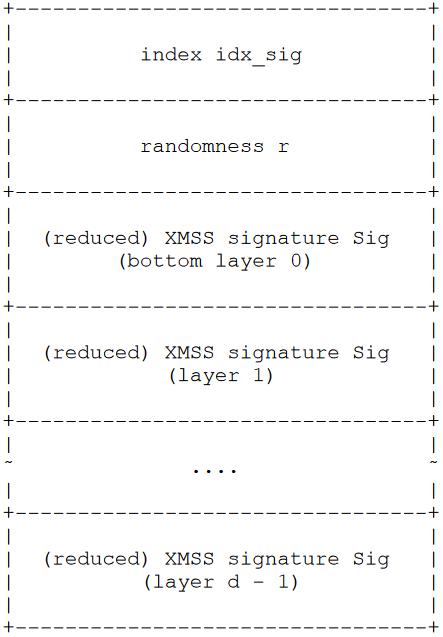
\includegraphics[width=\linewidth]{fig/MTsignature.png}
          \caption{Multi-tree signature}
          \label{fig:MTsig}
          
        \end{subfigure}%
        \begin{subfigure}{0.5\textwidth}
          \centering
          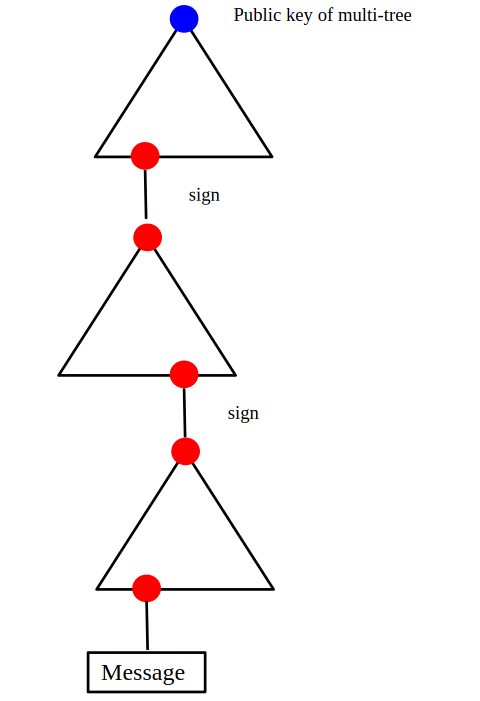
\includegraphics[width=\linewidth]{fig/multi-tree.png}
          \caption{Multi-tree general structure}
          \label{fig:MTstruc}
          
        \end{subfigure}
        \caption{$\text{XMSS}^{MT}$ multi-tree structure with $d$ layers, each containing subtrees of height $h'$. (a)~The multi-tree signature consists of $d$ XMSS signatures, one per layer. (b)~The overall hypertree: each subtree at layer $j$ signs the root of a subtree at layer $j{-}1$. For example, with $h = 20$ and $d = 4$, each subtree has height $h' = 5$, supporting $2^{20}$ total signatures.}
        \label{fig:LAT}
        \end{figure}


        
    \end{subsection}

    \begin{subsection}{Tree Traversal}

    A practical challenge in implementing XMSS and $\text{XMSS}^{MT}$ is the efficient computation of authentication paths. A na\"ive approach would require storing all $2^h$ leaves or recomputing them for each signature, which is prohibitive for large trees.

    The \textbf{BDS (Buchmann--Dahmen--Schneider) traversal algorithm} \cite{buchmann2013security} addresses this by maintaining a small set of precomputed nodes and updating them incrementally as signatures are generated. The key idea is to use a combination of:
    \begin{itemize}
        \item \textbf{Treehash instances}: background computations that prepare upcoming authentication path nodes before they are needed.
        \item \textbf{Retain stack}: a small stack storing nodes that would be expensive to recompute later.
        \item \textbf{Keep array}: nodes from the current authentication path that will be needed in future paths.
    \end{itemize}

    The BDS algorithm achieves a time complexity of $O(h / 2)$ hash computations per signature update and requires $O(h)$ storage for the traversal state. The XMSS RFC~\cite{huelsing2018rfc} specifies a variant of this algorithm as the recommended traversal strategy.

    For $\text{XMSS}^{MT}$, traversal is performed independently within each subtree of height $h'$, and a new subtree is initialized only when the current one is exhausted, further reducing the per-signature cost.

    \end{subsection}
\end{section}

\begin{section}{SPHINCS+}

    SPHINCS+ \cite{gaithersburgmdnist_2024_stateless} is one of the three signature algorithms standardized by NIST (published as FIPS 205 / SLH-DSA in 2024). Structurally, it is very similar to XMSS. Fundamentally, there are two main differences. First, the SPHINCS+ algorithm does not use an L-tree structure. Instead, it transforms WOTS+ public keys into a single public key by applying a hash function (see Section~\ref{sec:L-tree}). Second, unlike XMSS, which contains only a WOTS+ signature, the SPHINCS+ algorithm also includes a FORS signature layer underneath the WOTS+ signature. Since the FORS signature algorithm is a \emph{few-time} signature, it tolerates the possibility of signing multiple messages with the same key pair (see Section~2.8 for details). For this reason, SPHINCS+ is a stateless algorithm. Before each signing operation, it pseudorandomly selects an index (derived from a hash of the message) and generates the signature and authentication path from the part of the tree corresponding to that index. Because it does not require securely storing and updating state information, stateless SPHINCS+ offers a significant advantage over XMSS in this regard. However, the FORS layer, which makes SPHINCS+ stateless, adds an additional layer of signature under WOTS+, thereby increasing the signature size compared to XMSS. Note that while both XMSS and SPHINCS+ use tree-based structures, their public key sizes are not necessarily identical and depend on the specific parameter sets chosen (e.g., security level, hash function). Figure \ref{fig:SPHINCS} illustrates the general structure of the SPHINCS+ algorithm. 
    \begin{subsection}{SPHINCS+ Parameters}
        Parameters and their descriptions are given below: 
    \begin{description}
  \item[$n$:] Hash output size in bits. All outputs of the underlying hash functions (e.g., $H_{\mathrm{msg}}$, PRF, and Merkle-node hashes) are exactly $n$ bits long.
  
  \item[$w$:] Winternitz parameter. Determines the base for WOTS\texttt{+} chains.  
    Higher $w$ reduces signature length at the cost of more hash computations per chain.

  \item[$\ell$:] Total number of $n$-bit chains in each WOTS\texttt{+} key or signature, given by


\[
    \ell = \ell_1 + \ell_2,
    \quad
    \ell_1 = \left\lceil \frac{8n}{\log_2 w} \right\rceil,
    \quad
    \ell_2 = \left\lfloor \frac{\log_2(\ell_1\,(w-1))}{\log_2 w} \right\rfloor + 1.
  \]

  \item[$h$:] Total height of the Merkle hypertree.  
    The overall number of leaves (XMSS key pairs) is $2^h$.

  \item[$h'$:] Height of each XMSS subtree.  
    Each subtree contains $2^{h'}$ leaves, and we arrange $d$ such layers to reach height $h$.

  \item[$d$:] Number of layers in the hypertree, satisfying
  
\[
    d = \frac{h}{h'}.
  \]

  \item[$k$:] Number of parallel FORS trees.  
    The $n$-bit message digest is split into $k$ indices, each signed by one FORS tree.
\end{description}
    \end{subsection}
    


    \begin{figure}[H]
        \centering
        % Private Key Table
        \begin{minipage}{0.45\textwidth}
        \centering
        \begin{tabular}{|l|l|}
        \hline
        \textbf{SK.seed} & $n$ bytes \\
        \hline
        \textbf{SK.prf}  & $n$ bytes \\
        \hline
        \textbf{PK.seed} & $n$ bytes \\
        \hline
        \textbf{PK.root} & $n$ bytes \\
        \hline
        \end{tabular}
        \caption{SPHINCS+ private key}
        \label{fig:slhdsa_privatekey}
        \end{minipage}
        \hfill
        % Public Key Table
        \begin{minipage}{0.45\textwidth}
        \centering
        \begin{tabular}{|l|l|}
        \hline
        \textbf{PK.seed} & $n$ bytes \\
        \hline
        \textbf{PK.root} & $n$ bytes \\
        \hline
        \end{tabular}
        \caption{SPHINCS+ public key}
        \label{fig:slhdsa_publickey}
        \end{minipage}
        
    \end{figure}


    \begin{figure}
        \centering
        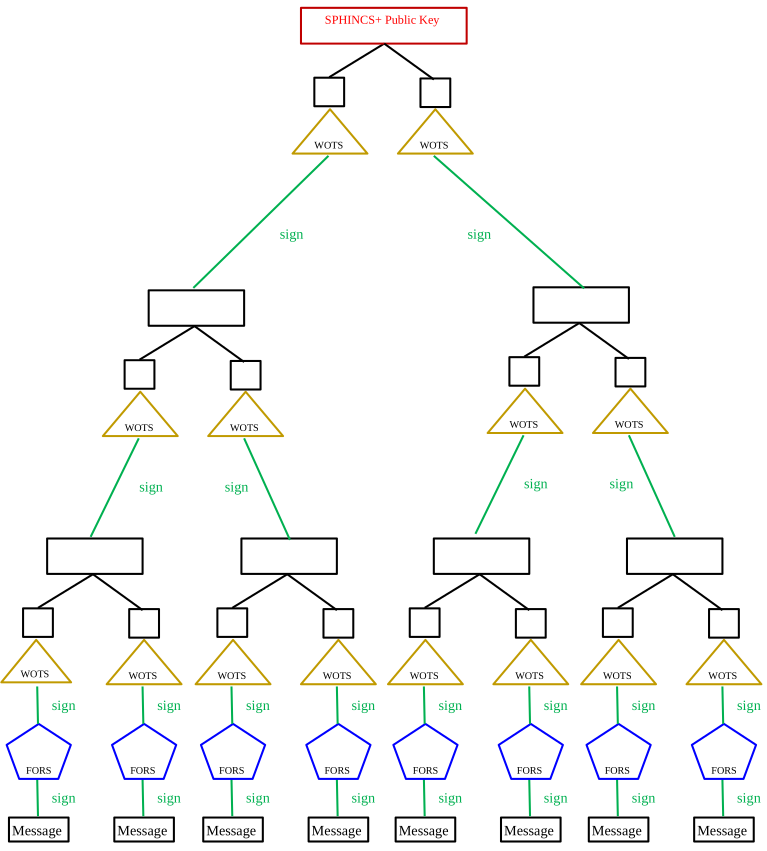
\includegraphics[width=1.1\linewidth]{fig/sphıncs.png}
        \caption{SPHINCS+ General structure}
        \label{fig:SPHINCS}
    \end{figure}


\begin{subsection}{SPHINCS+ Key Generation}

Key generation derives a full SPHINCS+ key pair from three seeds: the secret seed, the PRF key, and the public seed. It first initializes the ADRS value with a zero‐filled 32‐byte string and configures it for the top-level XMSS tree by setting the layer address to \(d-1\). The root node of that tree is computed via a single call to \texttt{xmss\_node}, which absorbs the secret seed, the public seed, and the ADRS state. Finally, the algorithm returns the secret key tuple \((\mathit{SK}.\mathit{seed},\,\mathit{SK}.\mathit{prf},\,\mathit{PK}.\mathit{seed},\,\mathit{PK}.\mathit{root})\) alongside the public key \((\mathit{PK}.\mathit{seed},\,\mathit{PK}.\mathit{root})\) (see Algorithm~\ref{alg:sphincs_keygen}).

\begin{algorithm}
\caption{SPHINCS\_keyGen -- Generate a SPHINCS+ key pair}
\label{alg:sphincs_keygen}

\textbf{Input:} None \\
\textbf{Output:} SPHINCS+ private key \texttt{SK}, SPHINCS+ public key \texttt{PK}

\vspace{0.3cm}

\begin{tabular}{ll}
1: & Generate uniformly random $n$-byte strings: \texttt{SK.SEED}, \texttt{SK.PRF}, \texttt{PK.SEED} \\
2: & Initialize \texttt{ADRS} as a zeroed address structure \\
3: & \texttt{PK.root} $\leftarrow$ \texttt{treehash(SK\_SEED, PUB\_SEED, ADRS)} \\
4: & \texttt{SK} $\leftarrow$ \texttt{SK.SEED $\parallel$ SK.PRF $\parallel$ PUB.SEED $\parallel$ PK.root} \\
5: & \texttt{PK} $\leftarrow$ \texttt{PK.SEED $\parallel$ PK.root} \\
6: & \textbf{return} \texttt{SK, PK}
\end{tabular}
\end{algorithm}

\end{subsection}

\begin{subsection}{SPHINCS+ Sign}

Signature generation begins by initializing the ADRS to zero and optionally randomizing the message randomizer input. The PRF keyed by \(\mathit{SK}.\mathit{prf}\) produces the randomness \(R\) that is prepended to the signature. A message digest is then computed over \(R\), the public seed, the root, and the message itself. This digest is split into the message digest bits \(\mathit{md}\) and the tree/leaf indices \(\mathit{idx\_tree},\mathit{idx\_leaf}\). The FORS scheme is applied at the lowest layer (layer 0) to sign \(\mathit{md}\), yielding \(\mathit{SIG\_FORS}\) and an authenticated public key \(\mathit{PK\_FORS}\). Finally, the hypertree (HT) signature over \(\mathit{PK\_FORS}\) is computed and appended, producing the full SPHINCS+ signature (see Algorithm~\ref{alg:spx_sign})

\begin{algorithm}
    \caption{spx\_sign -- Generating a SPHINCS+ signature}
    \label{alg:spx_sign}
    \textbf{Input:} Message \texttt{M}, private key \texttt{SK} = (\texttt{SK.seed}, \texttt{SK.prf}, \texttt{PK.seed}, \texttt{PK.root}) \\
    \textbf{Output:} SPHINCS+ signature \texttt{SIG}

    \vspace{0.2cm}

    \begin{tabular}{ll}
    1:  & \texttt{ADRS} $\leftarrow$ \texttt{toByte(0, 32)} \\
    2:  & \texttt{opt}  $\leftarrow$ \texttt{PK.seed} \\
    3:  & \textbf{if} \texttt{RANDOMIZE} \textbf{then} \\
    4:  & \quad \texttt{opt}  $\leftarrow$ \texttt{rand(n)} \\
    5:  & \textbf{end if} \\
    6:  & \texttt{R}    $\leftarrow$ \texttt{PRF\_msg(SK.prf, opt, M)} \\
    7:  & \texttt{SIG}  $\leftarrow$ \texttt{R} \\
    8:  & \texttt{digest} $\leftarrow$ \texttt{H\_msg(R, PK.seed, PK.root, M)} \\
    9:  & \texttt{tmp\_md}       $\leftarrow$ first $\lfloor(\mathit{ka}+7)/8\rfloor$ bytes of \texttt{digest} \\
    10: & \texttt{tmp\_idx\_tree} $\leftarrow$ next $\lfloor(h - h/d +7)/8\rfloor$ bytes of \texttt{digest} \\
    11: & \texttt{tmp\_idx\_leaf} $\leftarrow$ next $\lfloor(h/d +7)/8\rfloor$ bytes of \texttt{digest} \\
    12: & \texttt{md}      $\leftarrow$ first \texttt{ka} bits of \texttt{tmp\_md} \\
    13: & \texttt{idx\_tree} $\leftarrow$ first $(h - h/d)$ bits of \texttt{tmp\_idx\_tree} \\
    14: & \texttt{idx\_leaf} $\leftarrow$ first $h/d$ bits of \texttt{tmp\_idx\_leaf} \\
    15: & \texttt{ADRS.setLayerAddress(0)} \\
    16: & \texttt{ADRS.setTreeAddress(idx\_tree)} \\
    17: & \texttt{ADRS.setType(FORS\_TREE)} \\
    18: & \texttt{ADRS.setKeyPairAddress(idx\_leaf)} \\
    19: & \texttt{SIG\_FORS} $\leftarrow$ \texttt{fors\_sign(md, SK.seed, PK.seed, ADRS)} \\
    20: & \texttt{SIG}      $\leftarrow$ \texttt{SIG} \texttt{||} \texttt{SIG\_FORS} \\
    21: & \texttt{PK\_FORS} $\leftarrow$ \texttt{fors\_pkFromSig(SIG\_FORS, md, PK.seed, ADRS)} \\
    22: & \texttt{ADRS.setType(TREE)} \\
    23: & \texttt{SIG\_HT}   $\leftarrow$ \texttt{ht\_sign(PK\_FORS, SK.seed, PK.seed, idx\_tree, idx\_leaf)} \\
    24: & \texttt{SIG}      $\leftarrow$ \texttt{SIG} \texttt{||} \texttt{SIG\_HT} \\
    25: & \textbf{return} \texttt{SIG}
    \end{tabular}
\end{algorithm}



\begin{table}[ht]
  \centering
  \begin{tabular}{|l|}
    \hline
    \textbf{Signature}                         \\ \hline
    Randomness \(R\)                         \\ \hline
    FORS Signature \(\mathrm{SIG}_{\mathrm{FORS}}\)        \\ \hline
    HT Signature \(\mathrm{SIG}_{\mathrm{HT}}\)        \\ \hline
  \end{tabular}
  \caption{SPHINCS+ signature data format}
  \label{tab:slh-dsa-format}
\end{table}



\end{subsection}

\begin{subsection}{SPHINCS+ Verify}

Verification mirrors signing: it parses the incoming signature into \(R\), \(\mathit{SIG\_FORS}\), and \(\mathit{SIG\_HT}\). The verifier recomputes the message digest and splits it into \(\mathit{md}\), \(\mathit{idx\_tree}\), and \(\mathit{idx\_leaf}\). It then re-derives the FORS public key by running \(\mathit{fors\_pkFromSig}\) on \(\mathit{SIG\_FORS}\) and \(\mathit{md}\). Finally, the hypertree signature is checked with \(\mathit{ht\_verify}\), which returns \(\mathit{true}\) only if every component matches the stored public root (see Algorithm~\ref{alg:spx_verify}).

\begin{algorithm}
    \caption{spx\_verify -- Verify a SPHINCS+ signature SIG on a message M using a SPHINCS+ public key PK}
    \label{alg:spx_verify}
    \textbf{Input:} Message \texttt{M}, signature \texttt{SIG}, public key \texttt{PK} \\
    \textbf{Output:} Boolean

    \vspace{0.2cm}

    \begin{tabular}{ll}
        1:  & \texttt{ADRS} $\leftarrow$ \texttt{toByte(0, 32)} \\
        2:  & \texttt{R} $\leftarrow$ \texttt{SIG.getR()} \\
        3:  & \texttt{SIG\_FORS} $\leftarrow$ \texttt{SIG.getSIG\_FORS()} \\
        4:  & \texttt{SIG\_HT} $\leftarrow$ \texttt{SIG.getSIG\_HT()} \\
        5:  & \texttt{digest} $\leftarrow$ \texttt{H\_msg(R, PK.seed, PK.root, M)} \\
        6:  & \texttt{tmp\_md} $\leftarrow$ first $\lfloor(\mathit{ka}+7)/8\rfloor$ bytes of \texttt{digest} \\
        7:  & \texttt{tmp\_idx\_tree} $\leftarrow$ next $\lfloor(h - h/d +7)/8\rfloor$ bytes of \texttt{digest} \\
        8:  & \texttt{tmp\_idx\_leaf} $\leftarrow$ next $\lfloor(h/d +7)/8\rfloor$ bytes of \texttt{digest} \\
        9:  & \texttt{md} $\leftarrow$ first \texttt{ka} bits of \texttt{tmp\_md} \\
        10: & \texttt{idx\_tree} $\leftarrow$ first $(h - h/d)$ bits of \texttt{tmp\_idx\_tree} \\
        11: & \texttt{idx\_leaf} $\leftarrow$ first $h/d$ bits of \texttt{tmp\_idx\_leaf} \\
        12: & \texttt{ADRS.setLayerAddress(0)} \\
        13: & \texttt{ADRS.setTreeAddress(idx\_tree)} \\
        14: & \texttt{ADRS.setType(FORS\_TREE)} \\
        15: & \texttt{ADRS.setKeyPairAddress(idx\_leaf)} \\
        16: & \texttt{PK\_FORS} $\leftarrow$ \texttt{fors\_pkFromSig(SIG\_FORS, md, PK.seed, ADRS)} \\
        17: & \texttt{ADRS.setType(TREE)} \\
        18: & \textbf{return} \texttt{ht\_verify(PK\_FORS, SIG\_HT, PK.seed, idx\_tree, idx\_leaf, PK.root)} \\
    \end{tabular}
\end{algorithm}


\end{subsection}
\end{section}

\begin{section}{LMS and HSS}

The \textbf{Leighton--Micali Signature (LMS)} scheme \cite{mcgrew2019leighton} is a stateful hash-based signature algorithm standardized in IETF RFC~8554. Like XMSS, LMS is built from a one-time signature component combined with a Merkle tree to support multiple signatures. Its multi-tree extension is called \textbf{HSS (Hierarchical Signature System)}, analogous to $\text{XMSS}^{MT}$.

\subsection{LMS Construction}

LMS uses the \textbf{Leighton--Micali One-Time Signature (LM-OTS)} as its underlying OTS scheme. LM-OTS operates similarly to WOTS: the message digest is divided into $p$ chunks in base $2^w$, and each chunk determines how many times a hash chain is iterated. The key differences from WOTS+ are:

\begin{itemize}
    \item \textbf{Randomized hashing:} LM-OTS uses a different randomization approach. Instead of XOR-based bitmasking (as in WOTS+), LM-OTS prepends a diversification string (the OTS type identifier, the key identifier, the leaf index $q$, and a chain index $i$) to each hash input, achieving domain separation through message formatting rather than XOR masking.
    \item \textbf{Final hash:} After computing all $p$ chain values, LM-OTS concatenates them and applies a final hash to produce a single $n$-byte value that serves as the OTS public key. WOTS+ uses an L-tree for this compression step in XMSS.
\end{itemize}

The LMS Merkle tree is constructed over $2^h$ LM-OTS public keys (where $h$ is the tree height), and the LMS public key is the root of this tree. Signing uses the $q$-th OTS key pair and includes the authentication path. Verification reconstructs the root from the OTS signature and checks it against the stored public key.

\subsection{HSS: Multi-Tree Extension}

HSS extends LMS to a multi-tree (hypertree) structure with $L$ levels, analogous to $\text{XMSS}^{MT}$. At each level $i$ ($i = 0, \ldots, L-1$), there is an LMS tree of height $h_i$. The top-level tree signs the public keys of the next level down, and the bottom level signs the actual messages. The total number of available signatures is $\prod_{i=0}^{L-1} 2^{h_i}$.

\subsection{Comparison of Standardized HBS Schemes}

Table~\ref{tab:hbs_comparison} provides a systematic comparison of the three standardized hash-based signature schemes.

\begin{table}[ht]
\centering
\renewcommand{\arraystretch}{1.3}
\caption{Comparison of standardized hash-based signature schemes}
\label{tab:hbs_comparison}
\begin{tabular}{|l|c|c|c|}
\hline
\textbf{Property} & \textbf{LMS/HSS} & \textbf{XMSS/$\text{XMSS}^{MT}$} & \textbf{SPHINCS+} \\
\hline
\textbf{Standard} & RFC 8554 & RFC 8391 & FIPS 205 (SLH-DSA) \\
\hline
\textbf{Statefulness} & Stateful & Stateful & Stateless \\
\hline
\textbf{OTS Scheme} & LM-OTS & WOTS+ & WOTS+ + FORS \\
\hline
\textbf{Randomization} & Domain separation & XOR bitmask & Tweakable hash \\
\hline
\textbf{PK Compression} & Final hash & L-tree & Hash of concat. \\
\hline
\textbf{Multi-tree} & HSS ($L$ levels) & $\text{XMSS}^{MT}$ ($d$ layers) & Hypertree ($d$ layers) \\
\hline
\textbf{Max Signatures} & $\prod 2^{h_i}$ & $2^h$ & Unlimited \\
\hline
\textbf{PK Size} & $2n + 24$ bytes & $2n + 4$ bytes (OID) & $2n$ bytes \\
\hline
\textbf{Sig. Size (128-bit)} & $\approx$2--4 KB & $\approx$2--3 KB & $\approx$7--50 KB \\
\hline
\textbf{Security Assumption} & PRF, 2nd-preimage & PRF, 2nd-preimage & PRF, multi-target \\
\hline
\end{tabular}
\end{table}

\textbf{Key observations:}
\begin{itemize}
    \item LMS/HSS and XMSS/$\text{XMSS}^{MT}$ are both stateful and produce compact signatures, but require careful state management to avoid catastrophic key reuse.
    \item SPHINCS+ eliminates state management at the cost of significantly larger signatures (due to the FORS layer and deeper hypertree).
    \item The choice of domain separation mechanism (XOR bitmask in XMSS vs.\ input formatting in LMS) leads to slightly different security proofs but comparable security guarantees.
    \item For applications where state can be securely managed (e.g., firmware signing, secure boot), LMS or XMSS are preferred due to their smaller signatures. For general-purpose applications, SPHINCS+ is the safer choice.
\end{itemize}

\end{section}

\begin{section}{Some Attacks on Hash-Based Signatures}

This section examines several notable attacks on hash-based signature algorithms. For each attack, we present the attack model, the construction, the applicable schemes, the complexity, and known countermeasures.

\subsection{Intermediate Value Guessing Attack}

This attack was defined in the paper by Booth et al.\cite{booth2021intermediate}. In the document by H\"ulsing et al. \cite{huelsing2018rfc}, it is stated that the secret key values used in the WOTS+ signature must be generated in a uniformly distributed manner, but the specific generation method is left to the implementer.

We first introduce the notation used in this section. Let $\mathit{osk}$ (\textit{OTS secret key}) denote the WOTS+ secret key for leaf index $i$, consisting of $\ell$ chain starting values. Let $F$ denote a pseudorandom function used to derive these values, and let $w$ denote the Winternitz parameter (so each base-$w$ digit ranges over $\{0, 1, \ldots, w{-}1\}$). A digit value of $0$ means the secret key element is used directly (without any hash iteration), while a digit value of $w{-}1$ (denoted $F$ in the base-$w$ representation) means the element is hashed $w{-}1$ times, yielding the public key component.

Assume that the WOTS+ secret keys ($\mathit{osk}$) are generated from the seed values $\texttt{seed}_{\text{OTS},i}$ as follows:

\[
\texttt{osk} = (x_{i,1}, x_{i,2}, \ldots, x_{i,l}) = (F(\texttt{seed}_{\text{OTS},i},1), \ldots, F(\texttt{seed}_{\text{OTS},i},l))
\]

Under this assumption:

\begin{itemize}
    \item The signatures of messages whose base-$w$ representation includes zero values leak the corresponding indices of \texttt{osk}. For instance, if the base-$w$ representation of message $M$ is $BM = (b_1, 0, b_2)$, then the signature $\sigma_M = (Z_1, x_{i,2}, Z_3)$ reveals $x_{i,2}$. (Here, each $Z$ value is derived by applying the hash algorithm to a secret key index $w$ times.)
    
    \item The \texttt{osk} values used to sign different messages are generated from different seed values.
    
    \item Using a different seed for each WOTS+ secret key allows a multi-target attack, as described below.
\end{itemize}

In this attack, the adversary proceeds as follows:

\begin{itemize}
    \item Executes the signing oracle to obtain multiple WOTS+ message-signature pairs.
    \item Filters out pairs where fewer than two \texttt{osk} values are revealed.
    \item Assumes that a signature has the form $\sigma = (Z_1, \ldots, Z_l)$ and the message base-$w$ representation is $BM = (b_1, \ldots, b_l)$. The adversary identifies two indices $k_1$ and $k_2$ such that $Z_1$ and $Z_2$ correspond to $x_{i,k_1}$ and $x_{i,k_2}$ respectively. (Here, $k_1$ and $k_2$ are the positions where the base-$w$ value is zero.)
    
    \item From this, the adversary learns:
    \[
    x_{i,k_1} = F(\texttt{seed}_{\text{OTS},i}, k_1), \quad x_{i,k_2} = F(\texttt{seed}_{\text{OTS},i}, k_2)
    \]
    
    \item Using these values, the adversary constructs tables from message-signature pairs (assuming layer $j$ is known):
    \[
    (x_{k_1,k_2}, x_{k_2,i}, j), \quad (x_{k_3,k_4}, x_{k_4,i}, j)
    \]
    
    \item For each guessed \texttt{seed\textsubscript{OTS},i}, the adversary reconstructs a candidate $\texttt{osk}'$ and checks whether the generated value matches existing entries in the table. If both $x_{k_1}$ and $x_{k_2}$ match, the guess for $\texttt{seed\textsubscript{OTS},i}$ is considered correct.
\end{itemize}

Assuming the adversary correctly guesses $\texttt{seed}_{\text{OTS},i}$, let the message $M_i$ have the following XMSSMT signature structure. To forge a valid signature, the adversary uses one of the following strategies:

\paragraph{Case 1: Seed Belongs to Layer 0}

At layer 0, the signature is generated by signing $H(R \,\|\, \texttt{ROOT} \,\|\, i, M_i)$. Let $M_j$ be the adversary’s chosen message. The adversary computes $H(R \,\|\, \texttt{ROOT} \,\|\, i, M_j)$, signs it with the recovered secret key, and replaces the original signature value with this forged one. The authentication path values (\texttt{Auth}) remain unchanged, as they depend on the secret key used, not the signed message.

\paragraph{Case 2: Seed Belongs to Layer $j > 0$}

Suppose the recovered seed belongs to a WOTS+ instance at layer $j > 0$. In this case, the WOTS+ signs the root of layer $j-1$. In XMSSMT, signature verification is performed by computing the root at each layer and comparing the top-layer root with the public key. If the seed belongs to a layer $j > 0$, the adversary can forge the subtree below layer $j$ for a chosen message, replacing the signature value at layer $j$ while keeping the rest of the signature unchanged. Since the upper layers remain valid, the signature is accepted as legitimate.

\begin{figure}
    \centering
    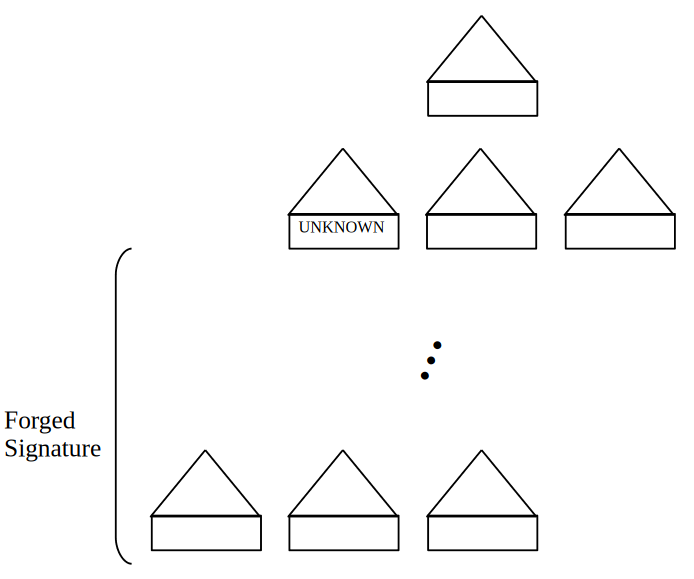
\includegraphics[width=0.5\linewidth]{fig/inter_secr_guess.png}
    \caption{Intermediate Value Guessing: the adversary recovers OTS seed values from observed signatures and uses them to forge signatures at the corresponding tree layer.}
    \label{fig:intermediateValueGuessing}
\end{figure}

\textbf{Impact and Countermeasures.}
This attack targets XMSS$^{MT}$ implementations where WOTS+ secret keys are generated deterministically from per-leaf seeds using a simple PRF construction. The attack complexity depends on the number of observable signatures and the probability of zero-valued base-$w$ digits. \textbf{Countermeasure:} The attack is prevented by deriving each element of the WOTS+ secret key \emph{independently} from the master seed using a PRF that incorporates the chain index, i.e., $\mathit{sk}_{i,j} = \mathrm{PRF}(\mathit{SK.seed}, \mathit{ADRS}_{i,j})$, where the address includes both the OTS index and the chain index. This ensures that recovering one chain value does not reveal the seed and, hence, other chain values.

\subsection{Antonov's Attack}

\begin{figure}
    \centering
    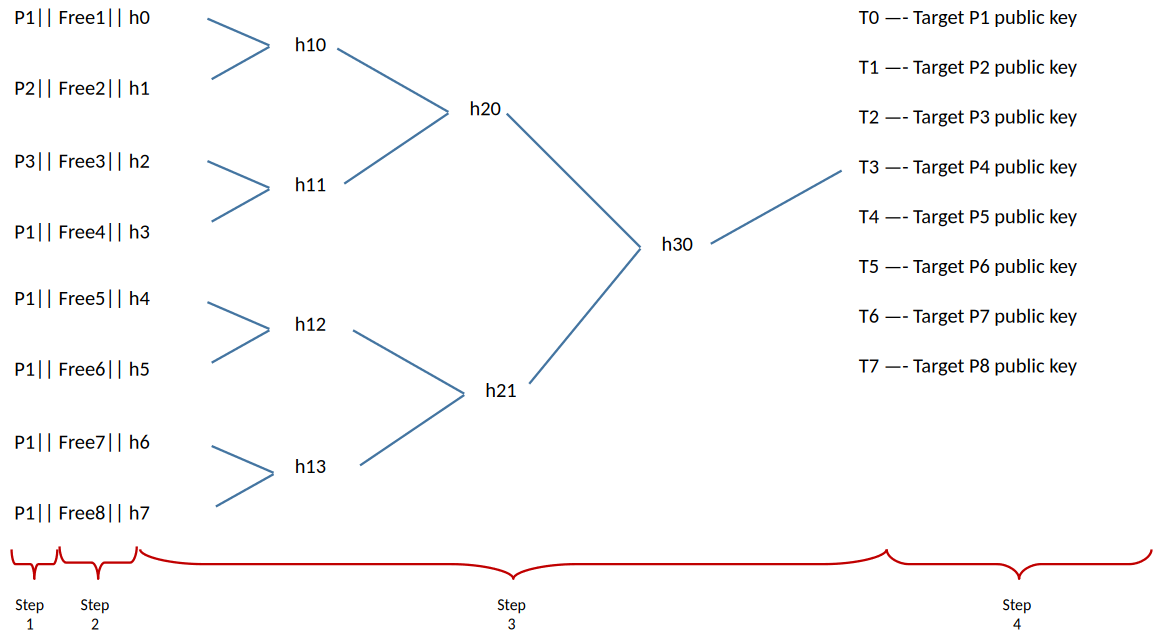
\includegraphics[width=\linewidth]{fig/antonov.png}
    \caption{Antonov's Attack}
    \label{fig:antonov}
    \label{fig:collision_steps}
\end{figure}

    The attack described in \cite{perlner2022breaking} exploits the Merkle–Damgård construction of the SHA-256 algorithm. Assume there are six target messages \( M_0, \ldots, M_5 \). For each message, different address values \( \text{ADRS}_0, \ldots, \text{ADRS}_5 \) are used within the hash algorithm. At this stage, intermediate values of the compression function \( C \) are obtained for each address.

Then, by applying a collision attack, the adversary finds random values \( x_0, \ldots, x_5 \), and captures pairwise collisions for the next set of intermediate values.

At this point, using the randomly found values \( X_{0,1}, X_{2,3}, X_{4,5} \), a 3-branch collision is constructed.

As the final step, the adversary finds a value \( Z \) such that the following equation holds for some \( i \in \{0,\ldots,5\} \):
\[
\text{SHA-256}(\text{ADRS}_i \,\|\, x_i \,\|\, X_{j,k} \,\|\, Z) = \text{SHA-256}(\text{ADRS}_i \,\|\, M_i)
\]

For example, if the prediction is found for \( M_3 \), then the equation
\[
\text{SHA-256}(\text{ADRS}_3 \,\|\, x_3 \,\|\, X_{2,3} \,\|\, Z) = \text{SHA-256}(\text{ADRS}_3 \,\|\, M_3)
\]
is satisfied, thus completing the multi-target prediction attack.

The complexity of finding a prediction in the final stage for \( t \) target messages is approximately \( 2^{256}/t \) compression function calls. The cost of finding an \( n \)-way collision is also determined by the number of \( C \) function evaluations.

This attack is broken down into four stages, as illustrated in Figure \ref{fig:antonov} 

\paragraph{Step 1:}
In this phase, the adversary collects a number of message-signature pairs signed using the same hash-based signature algorithm. Since the WOTS+ public keys used in the signature can be derived from the signature itself, the adversary also obtains these public keys. The attacker prefers messages with low checksum values at this stage (as lower checksums increase the probability of having \( F \) digits in the base-\( w \) representation). Although all message-signature pairs share the same \( \text{PK.seed} \), each has a distinct ADRS. In Figure~\ref{fig:collision_steps}, \( P_1, \ldots, P_8 \) represent the ADRS and PK.seed values. Finally, the attacker sorts these values.

\paragraph{Step 2:}
Here, the attacker selects random values \( \text{sk}_1, \ldots, \text{sk}_n \) and computes their hashes \( 2w \) times. By concatenating these values, they obtain the aggregated WOTS+ public keys denoted as \( \text{free}_1, \ldots, \text{free}_8 \).

\paragraph{Step 3:}
The attacker appends random values \( h \) to the free values and uses the method explained at the beginning of this section to find an \( n \)-way collision. Unlike Stage 2, the attacker does not know the secret keys corresponding to the WOTS+ public keys in this step.

\paragraph{Step 4:}
In this stage, the attacker compares the found \( n \)-way collision value with the targeted public keys using the value \( h_{30} \). \( T_0, \ldots, T_7 \) represent the target public keys before the checksum is added. If a collision is detected, the attacker has successfully forged a new WOTS+ public key whose hash value matches that of a legitimate public key.

As a result of the above steps, the attacker can generate a forged signature with a fake key. In both SPHINCS+ and XMSS algorithms, public keys generated at each layer during verification are not checked directly—instead, their hash values are computed and passed on to the next layer. Therefore, even if the attacker’s keys differ from the legitimate keys, verification succeeds as long as the hash values match. The main constraint of this attack is that the message to be signed must follow a specific format:

\begin{center}
\texttt{XXXXXXXX XXXXXXXX XXXXXXXF FFFFFFFF FFFFFFFF FFFFFFFF FFFFFFFF FFFFFFFF}
\end{center}

(where \( X \) can be any value). This requirement arises because the attacker knows the secret keys corresponding to the public keys used in Stage 2, but not those in Stage 3. In WOTS+ signatures, the public key is used to sign positions marked with \( F \); therefore, message segments where the secret key is unknown must be fixed to \( F \) to successfully carry out the attack.

\textbf{Impact and Countermeasures.}
This attack demonstrates that the Merkle--Damg\r{a}rd internal structure of SHA-256 can be exploited in the context of HBS to reduce the cost of multi-target preimage searches. The attack is primarily theoretical and requires a very large number of signature queries. \textbf{Countermeasure:} Using hash functions that do not rely on the Merkle--Damg\r{a}rd construction (e.g., SHA-3/SHAKE) eliminates this attack vector. Additionally, choosing larger security parameters increases the attack complexity beyond practical feasibility.

\subsection{Fault Injection Attacks}

Fault injection attacks consist of scenarios in which one or more components of the algorithm are assumed to malfunction or operate incompletely due to external interference. For hash-based signature schemes, an example of a fault injection attack is described in the \cite{wagner2023faulting}.

The WOTS+ one-time signature algorithm divides the message to be signed into $w$-bit chunks and generates the signature value by repeatedly applying the hash function to the secret key as many times as the numerical value of each chunk. At this stage, an attacker can compute the hash of the signature value one more time (when the message is not $F$) to create a valid signature. To prevent this, a checksum value is appended to the message before signing. This checksum is calculated as $c = (w - 1 - m)$, where $m$ is the number of $w$-bit message chunks.

With this checksum, if the attacker computes extra hashes from the signature value, the checksum value decreases. Since the hash functions are designed to be resistant to preimage attacks, the attacker cannot compute the new checksum value. The attack described in \cite{wagner2023faulting} is based on the checksum calculation process malfunctioning due to an injected fault. If the checksum calculation does not work correctly, the attacker may generate a valid signature for a message of their choice.

\textbf{Impact and Countermeasures.}
Fault injection attacks are particularly relevant for embedded implementations of HBS (e.g., in smart cards or HSMs) where physical access may be possible. \textbf{Countermeasure:} Implementations should include redundant checksum computation and verification, execute critical operations multiple times and compare results, and employ hardware-level fault detection mechanisms (e.g., error-detecting codes, voltage glitch detectors).

\subsection{Multi-Target Attacks}

Multi-target attacks aim to find preimages when multiple output values of the used hash function are known. For a hash function with an $n$-bit output, the complexity of finding a preimage is $2^n$. In multi-target attacks, if $d$ different hash outputs are known, the complexity of finding a preimage reduces to $2^n / d$.

The XMSS and SPHINCS+ algorithms mitigate this situation by using keyed hash functions. In each usage of the hash function, different key and mask values are used, effectively differentiating the hash function for each operation and ensuring security against multi-target attacks.

\textbf{Impact and Countermeasures.}
Without mitigation, multi-target attacks can significantly reduce the effective security level of HBS schemes, since a tree of height $h$ exposes $2^h$ hash outputs. \textbf{Countermeasure:} Both XMSS and SPHINCS+ use \emph{tweakable hash functions} (via address-dependent keys or masks) to ensure that each hash evaluation is effectively independent, preventing the adversary from amortizing preimage searches across different tree positions. LMS/HSS achieves the same goal through input-formatting-based domain separation.

\subsection{Summary of Attacks}

Table~\ref{tab:attack_summary} summarizes the attacks discussed above.

\begin{table}[ht]
\centering
\renewcommand{\arraystretch}{1.3}
\caption{Summary of attacks on hash-based signature schemes}
\label{tab:attack_summary}
\begin{tabular}{|l|c|c|l|}
\hline
\textbf{Attack} & \textbf{Target} & \textbf{Type} & \textbf{Countermeasure} \\
\hline
Intermediate Value & XMSS$^{MT}$ & Key recovery & Independent PRF per chain \\
\hline
Antonov's Attack & SPHINCS+/XMSS & Forgery & Larger parameters, non-MD hash \\
\hline
Fault Injection & WOTS+ & Impl. attack & Redundant checksum verification \\
\hline
Multi-Target & All HBS & Generic & Tweakable/keyed hash functions \\
\hline
\end{tabular}
\end{table}



\end{section}

\section{Conclusion}

Hash-based signature schemes provide a mature and theoretically sound foundation for post-quantum digital signatures. Their security is grounded in the robustness of cryptographic hash functions, making them well-suited for a future where quantum adversaries may render traditional public-key cryptosystems obsolete. 

In this paper, we presented a comprehensive overview of hash-based signature constructions, starting from the foundational building blocks---Lamport signatures, Winternitz one-time signatures (WOTS/WOTS+), and Merkle trees---to the standardized schemes XMSS (RFC~8391), LMS (RFC~8554), and the stateless SPHINCS+ (FIPS~205 / SLH-DSA). We analyzed their structural differences, key components, and operational procedures, including the role of checksum mechanisms, address structures, and few-time signature schemes such as FORS. A systematic comparison of these three standardized schemes highlights the trade-offs between statefulness, signature size, and implementation complexity.

We also discussed several cryptanalytic threats specific to HBS schemes---intermediate value guessing, Antonov's multi-target preimage attack, fault injection attacks, and generic multi-target attacks---analyzing for each the attack model, applicable constructions, complexity, and known countermeasures. These analyses underscore the importance of careful implementation choices (e.g., independent per-chain key derivation, redundant checksum verification) and appropriate parameter selection.

Future work may focus on improving efficiency through optimized tree traversal algorithms, reducing signature sizes via tighter security proofs, exploring the integration of LMS and XMSS into hybrid signature schemes, and designing post-quantum transition strategies that combine the strengths of HBS with other post-quantum approaches such as lattice-based or code-based signatures.

% This sample uses bibtex rather than biblatex.
\bibliography{template}

% NOTES
% - Download abbrev3.bib and crypto.bib from https://cryptobib.di.ens.fr/
% - Use biblio.bib for additional references not in the cryptobib database.
%   If possible, take them from DBLP.

\end{document}
